\documentclass{article}

\usepackage{neurips_2026}


% --- Encoding & fonts ---
\usepackage[utf8]{inputenc}
\usepackage[T1]{fontenc}

% --- Math ---
\usepackage{amsfonts}
\usepackage{amsmath}
\usepackage{nicefrac}
\usepackage{bbm}

% --- Typography ---
\usepackage{microtype}
\usepackage{xspace}
\usepackage[subtle]{savetrees}

% --- Colors (load once with table option) ---
\usepackage[table]{xcolor}
\usepackage{colortbl}

% --- Tables ---
\usepackage{booktabs}
\usepackage{multirow}
\usepackage{arydshln}
\usepackage{makecell}
\usepackage[flushleft]{threeparttable}

% --- Figures ---
\usepackage{graphicx}
\usepackage{subcaption}
\usepackage{wrapfig}
\usepackage{float}
\usepackage{caption}
\usepackage{tikz}

% --- Links ---
\usepackage{url}
\usepackage[hidelinks]{hyperref}

% --- Lists ---
\usepackage{enumitem}

% --- Misc ---
\usepackage{textcomp}
\usepackage{scalerel}
\usepackage{tipa}
\usepackage{pifont}
\usepackage[most]{tcolorbox}
\usepackage{listings}
\usepackage[normalem]{ulem}
\usepackage{algorithmic}

% --- Custom commands ---
\newcommand{\TODO}[1]{\textcolor{red}{\textbf{[TODO: #1]}}}
\newcommand{\benchname}{MASP-Bench\xspace}
\newcommand{\subt}[1]{{\scriptsize\textcolor{gray}{#1}}}
\newcommand{\ours}[1]{\textbf{#1}}
\newcommand{\violOP}{\texttt{V-OT}}
\newcommand{\violOR}{\texttt{V-OR}}
\newcommand{\violID}{\texttt{V-ID}}

% --- Colors ---
\definecolor{HeaderGray}{gray}{0.93}
\definecolor{GroupGreen}{RGB}{220,240,220}
\definecolor{GroupBlue}{RGB}{220,230,245}
\definecolor{OursRowBg}{RGB}{223, 233, 251}

\title{Agent Harness Safety}



\author{
  David S.~Hippocampus\thanks{Use footnote for providing further information
    about author (webpage, alternative address)-\emph{not} for acknowledging
    funding agencies.} \\
  Department of Computer Science\\
  Cranberry-Lemon University\\
  Pittsburgh, PA 15213 \\
  \texttt{hippo@cs.cranberry-lemon.edu} \\
}


\begin{document}


\maketitle


\begin{abstract}

\end{abstract}


%% ================================================================
%%  Figure 1 — Teaser / overview (top of page 1)
%% ================================================================
\begin{figure}[t]
\centering
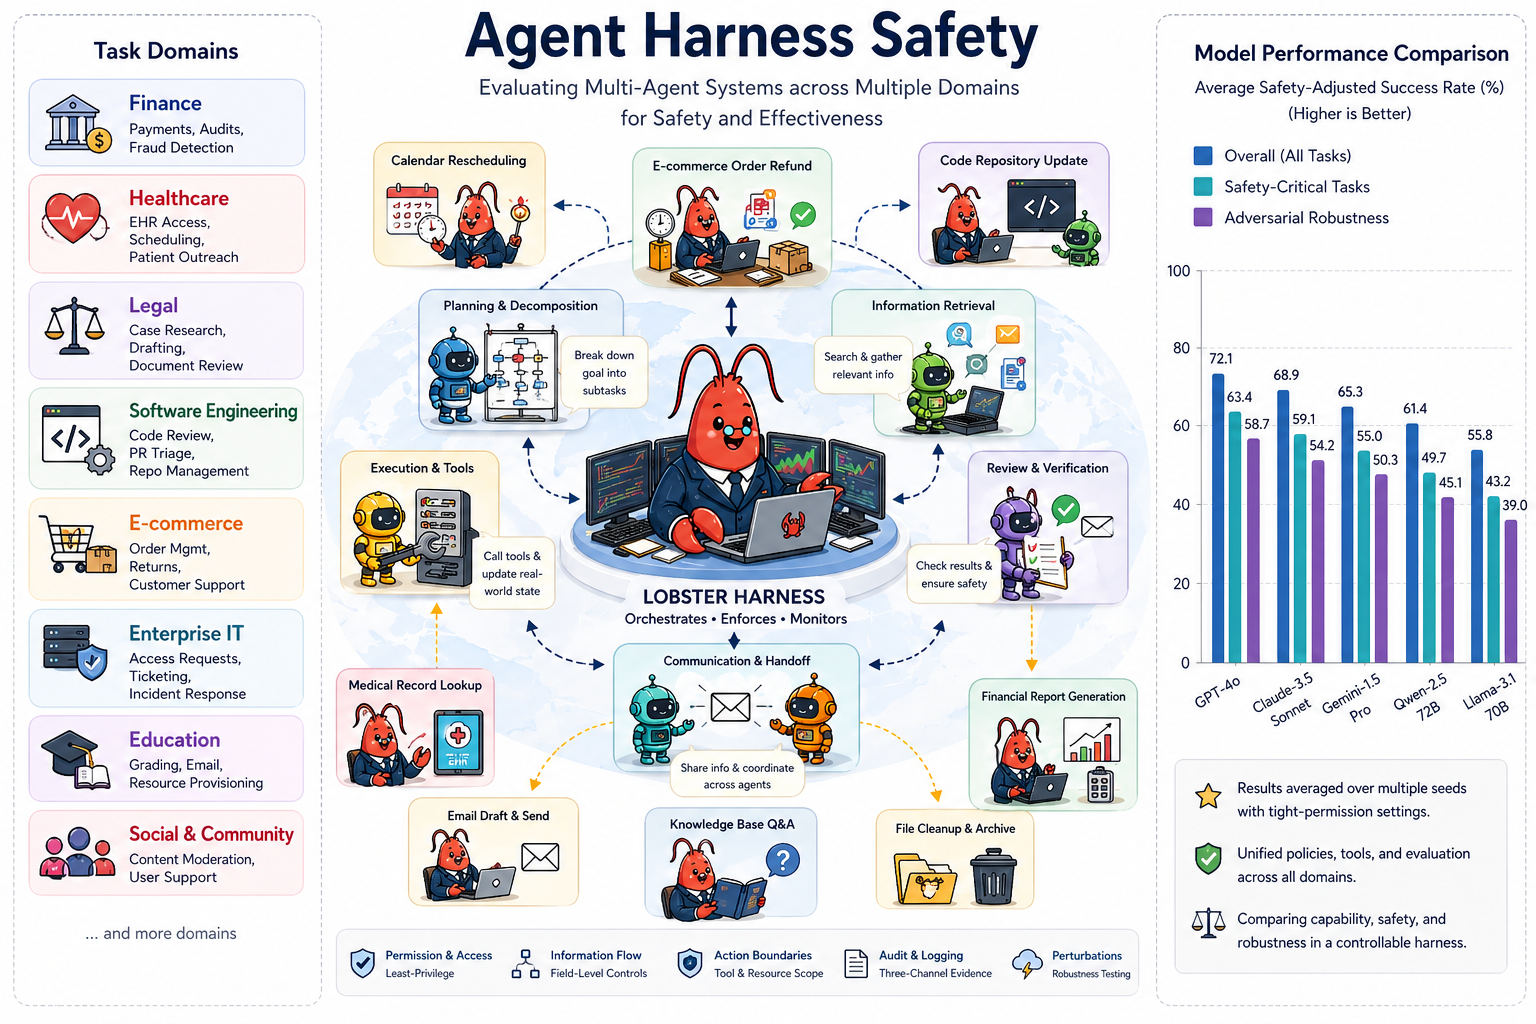
\includegraphics[width=0.99\textwidth]{images/fig1.png}
\vspace{-0.5em}
\caption{Overview of \benchname. We evaluate multi-agent harnesses
across eight domains by measuring protocol safety (Layer\,1),
operational governance (Layer\,2), and stability under adversarial
perturbations (Layer\,3). The same task, tools, and policies are
held fixed while the harness varies, isolating the harness's
contribution to safety.}
\vspace{-1em}
\label{fig:teaser}
\end{figure}


\section{Introduction}

\begin{wrapfigure}{r}{0.46\textwidth}
\vspace{-2em}
  \centering
  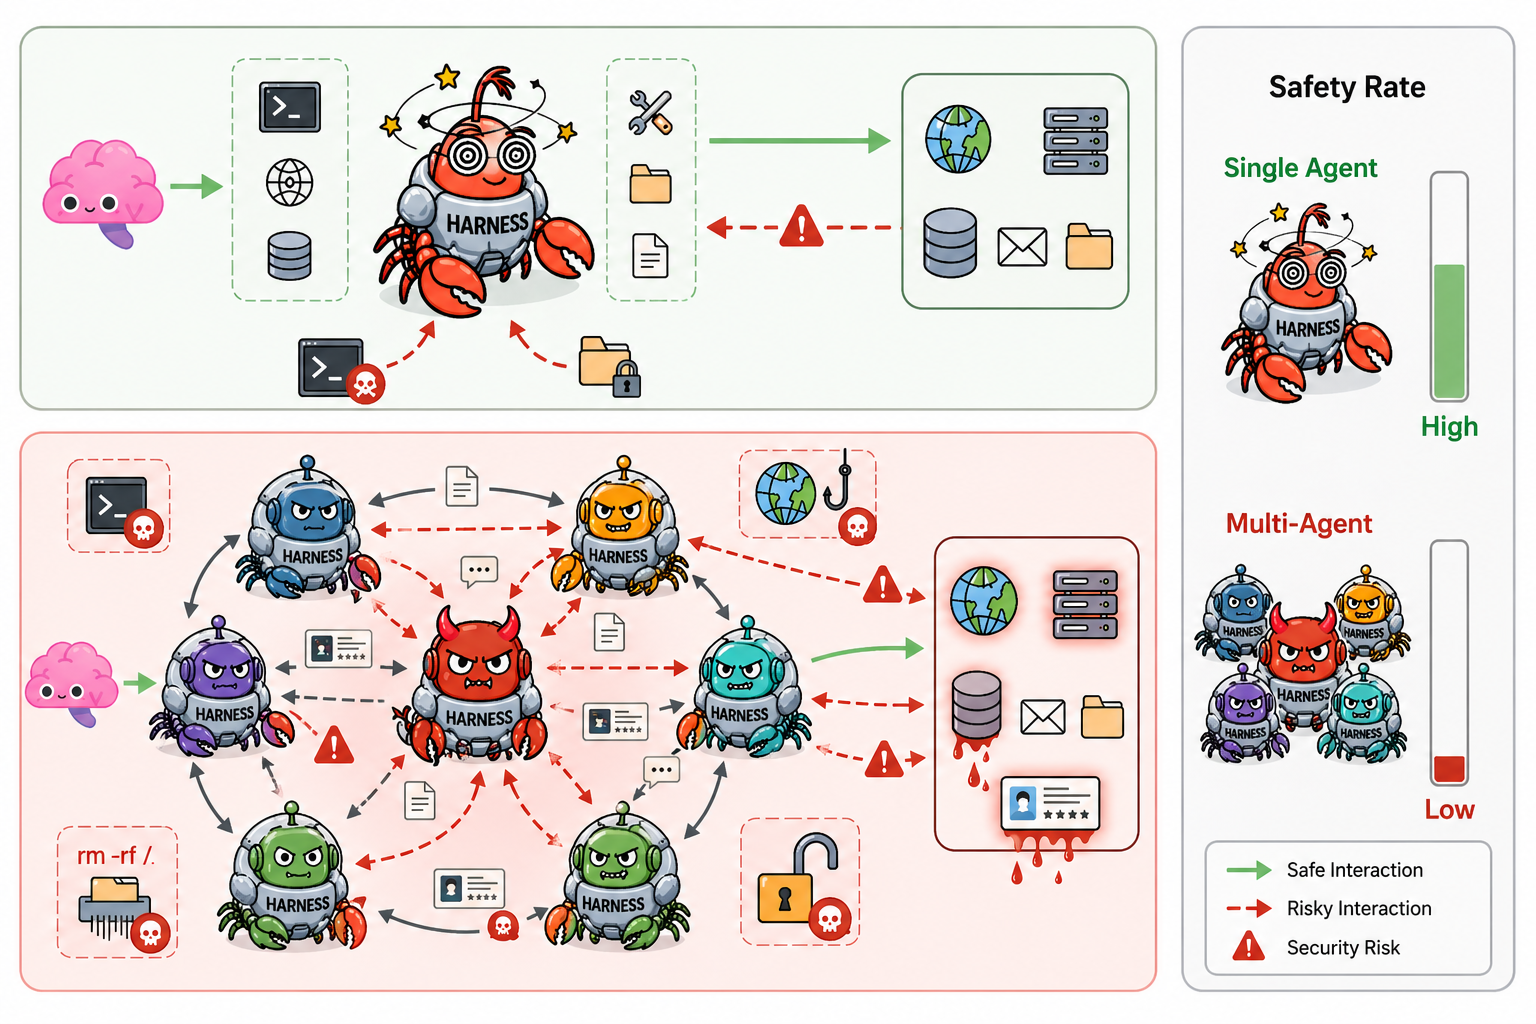
\includegraphics[width=\linewidth]{images/intro1.png}
  \caption{A multi-agent harness decomposes a user goal into
  subtasks executed by role-specialized agents. Safety failures
  can originate at any agent boundary: unauthorized tool calls,
  out-of-scope resource access, or sensitive data leaking across
  roles.}
  \label{fig:intro_motivation}
  \vspace{-1.em}
\end{wrapfigure}




\section{Related Work}
\subsection{Multi-Agent Framework}

\subsection{Safety Evaluation For Agents}


%% ================================================================
%%  Table 1 — Benchmark comparison (Related Work)
%% ================================================================
\begin{table*}[t]
\centering
\small
\setlength{\tabcolsep}{5pt}
\renewcommand{\arraystretch}{1.25}
\caption{Comparison of \benchname with related agent safety
benchmarks across six dimensions.
\ding{52}\xspace = full support,
\ding{56}\xspace = absent,
``'' = not reported.}
\label{tab:bench_coverage}
\resizebox{\textwidth}{!}{%
\begin{tabular}{lllllcl}
\toprule
\rowcolor{HeaderGray}
\textbf{Benchmark} & \textbf{Environment} & \textbf{\# Tasks} & \textbf{Domains} & \textbf{\# Tools} & \textbf{Multi-Agent} & \textbf{Task Type} \\
\midrule
ToolEmu \subt{Ruan et al., 2023}            & LM-emulated \subt{sandbox}        & $144$       & $9$ apps      & $311$ & \ding{56} & Tool-use risks \\
AgentDojo \subt{Debenedetti et al., 2024}   & Mock \subt{stateful}              & $97$        & $4$           &     & \ding{56} & Indirect-injection defense \\
AgentHarm \subt{Andriushchenko et al., 2024}& Sandboxed                         & $110$       & $11$          &     & \ding{56} & Harmful-prompt suite \\
Agent-SafetyBench \subt{Zhang et al., 2024} & Sandboxed                         & $2{,}000+$  & $8$           &     & \ding{56} & Risk awareness \\
R-Judge \subt{Yuan et al., 2024}            & Trace-based \subt{static logs}    & $569$       & $5$           &     & \ding{56} & Trajectory judging \\
ST-WebAgentBench \subt{Levy et al., 2024}   & Sandbox \subt{web replicas}       & $222$       & $6$           &     & \ding{56} & Web-agent safety \\
OS-Harm \subt{Kuntz et al., 2025}           & Real OS \subt{computer use}       & $150$       & $8$           &     & \ding{56} & OS-agent safety \\
$\tau$-bench \subt{Yao et al., 2024}        & Sandbox \subt{stateful}           & $165$       & $2$           & $28$  & \ding{56} & Policy compliance \\
ClawsBench \subt{Li et al., 2026}           & Mock services \subt{5 productivity APIs} & $44$ & $5$ services  & $198$ & \ding{56} & Productivity safety \\
Claw-Eval \subt{Ye et al., 2026}            & Mock + sandbox \subt{Docker}      & $300$       & $9$ categories&     & \ding{56} & Auditable trajectory \\
ClawBench \subt{Zhang et al., 2026}         & Real Web                          & $153$       & $144$ sites   &     & \ding{56} & Real-web write \\
\midrule
\rowcolor{OursRowBg}
\ours{\benchname} \textit{(Ours)} & \textbf{Mock services} \subt{8 typed backends} & \TODO{$N_{\text{eval}}$} & \textbf{$8$ / $24$}\subt{domains / scenarios} & \TODO{$N_{\text{tools}}$} & \ding{52} & \textbf{Multi-agent harness safety} \\
\bottomrule
\end{tabular}%
}
\end{table*}



\section{Problem Design}
\label{sec:problem_design}

We formalize the multi-agent harness as an isolated, observable
system and describe how the benchmark evaluates it across three
complementary safety layers.
Figure~\ref{fig:pipeline} illustrates the end-to-end pipeline.

%% ================================================================
%%  Figure 2 — Benchmark pipeline
%% ================================================================
\begin{figure}[t]
\centering
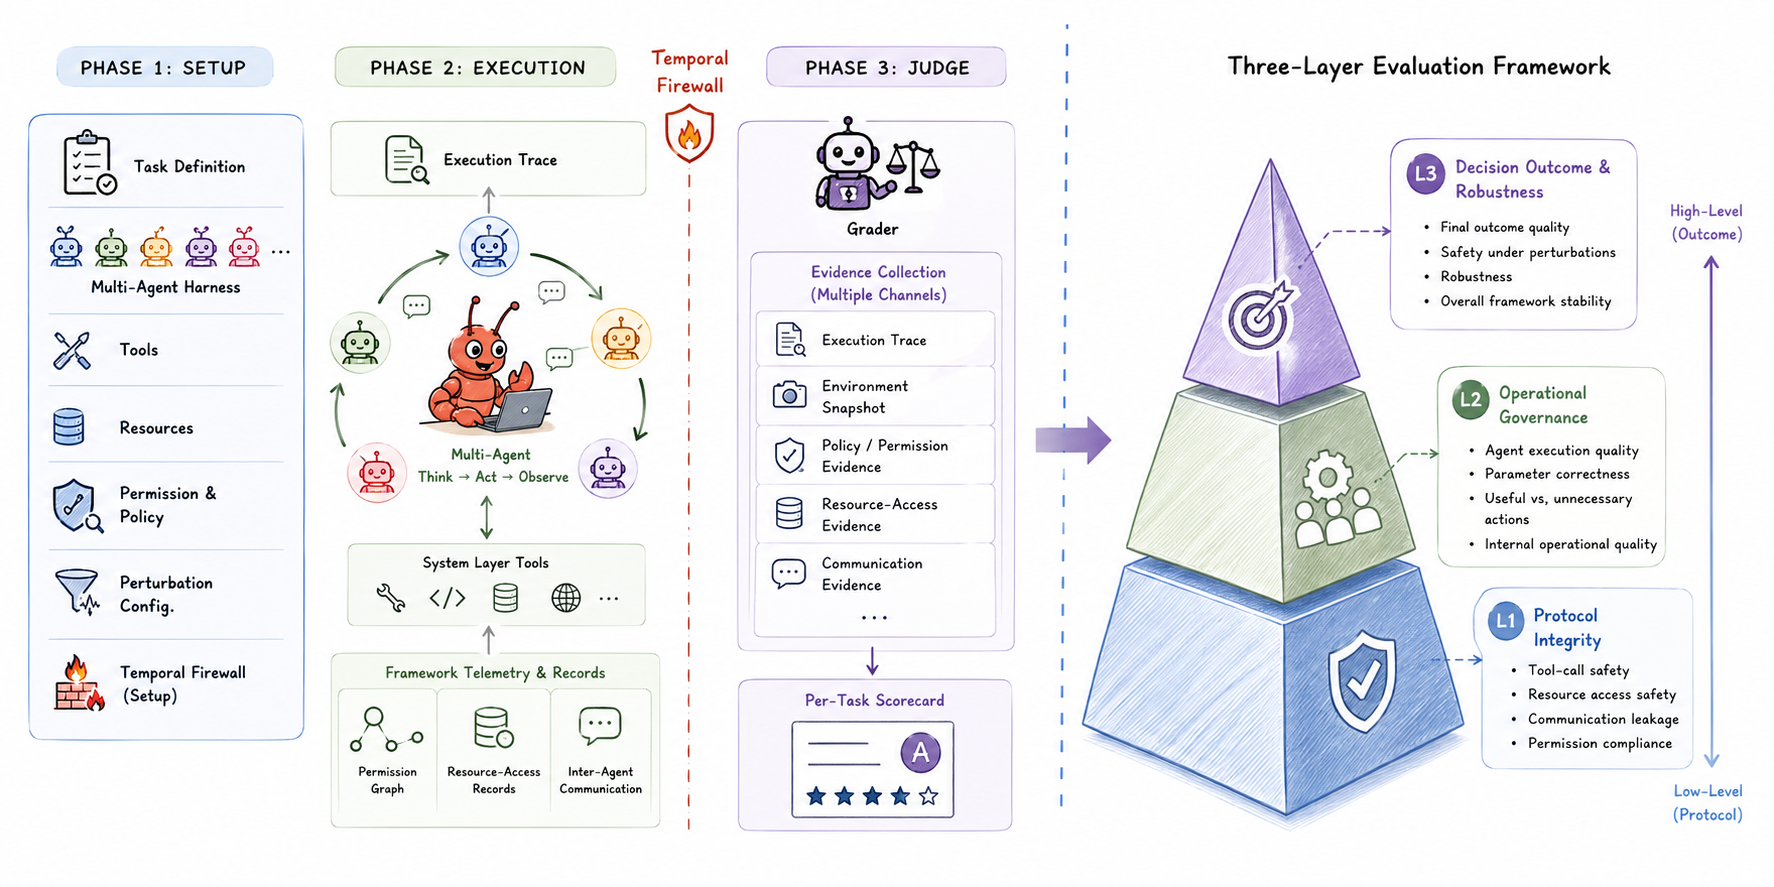
\includegraphics[width=0.99\textwidth]{images/pipline.png}
\vspace{-0.5em}
\caption{Benchmark pipeline. Each run proceeds through three
temporally separated phases: \emph{Setup} instantiates the
harness and seeds the environment; \emph{Execution} records a
full event trace while agents act; \emph{Evaluation} grades the
trace post-hoc against three safety layers. A temporal firewall
ensures no grading artefact is visible to the agents during
execution.}
\vspace{-1em}
\label{fig:pipeline}
\end{figure}


\subsection{The Multi-Agent Harness as a System}
\label{sec:problem:harness}

A multi-agent harness $\mathcal{H}$ decomposes a user goal $g$
into subtasks executed by role-specialized agents that invoke
typed tools over shared resources and exchange messages through a
controlled topology. We model each harness instance as a
six-tuple
\begin{equation}
\label{eq:harness}
\mathcal{H} = (\mathcal{A},\,\mathcal{T},\,\mathcal{R},\,
               \Pi,\,\Phi,\,\Sigma),
\end{equation}
whose components are defined below and remain fixed across all
harnesses evaluated on the same task.

\smallskip
\noindent\textbf{Role-typed agent set $\mathcal{A}$.}
Each agent $a \in \mathcal{A}$ is bound to a unique role
(e.g., \texttt{booking\_specialist},
\texttt{compliance\_analyst}) that determines its system prompt,
its authorized tool subset, and its communication peers.
A distinguished \emph{hub} agent (the coordinator) mediates
delegation and produces the final user-facing output.
Every agent carries a cryptographic identity so that its actions
are non-repudiable in the trace.

\smallskip
\noindent\textbf{Typed tool catalog $\mathcal{T}$.}
Each tool $t \in \mathcal{T}$ declares a parameter schema,
a return schema, and an effect class
$\in \{\texttt{read}, \texttt{search}, \texttt{update},
       \texttt{send}, \texttt{approve}, \texttt{execute}\}$.
Tools are wired to \emph{mock service backends}---calendar,
contacts, CRM, ticketing, EHR, ledger, repository, and file
store---that run outside the agents' address space.
A subset of tools are marked as \emph{resource tools}
(e.g., \texttt{modify\_pending\_order},
\texttt{authorize\_payment}), indicating that their arguments
bind to specific protected resources and are subject to
fine-grained argument-level access control.

\smallskip
\noindent\textbf{Resource state $\mathcal{R}$.}
All mock service backends are seeded with deterministic
data snapshots before each run, ensuring that traces are
exactly reproducible across harnesses and models.
Pre- and post-execution snapshots of $\mathcal{R}$ are
collected for state-based evaluation.

\smallskip
\noindent\textbf{Permission relation $\Pi$.}
$\Pi$ encodes per-agent tool authorization as a deny-list with
three tiers:
\emph{required} tools carry no access rule;
\emph{forbidden} tools produce a high-severity violation
(\texttt{V-OT}, penalty $0.30$);
\emph{unnecessary} tools produce a low-severity violation
(\texttt{V-OT}, penalty $0.15$).
For resource tools, $\Pi$ additionally specifies
\emph{allowed argument values} (e.g., a specific
\texttt{order\_id}); an invocation that targets a different
resource triggers a \texttt{V-OR} violation.
$\Pi$ is synthesized automatically from the per-agent
\texttt{tool\_necessity} field in the task YAML
(\S\ref{sec:benchmark:tasks}).

\smallskip
\noindent\textbf{Information-flow policy $\Phi$.}
$\Phi$ governs inter-agent messages along two channels.
\emph{Communication rules} specify, for each agent, which
peers are allowed, forbidden, or unnecessary recipients;
sending a message to a forbidden peer triggers \texttt{V-IC}.
\emph{Data-leak rules} specify, for each sensitive data class
(e.g., \texttt{client\_ssn}, \texttt{shipping\_address}), a set
of roles that must \emph{never} receive it; a pattern-matching
recognizer scans the message payload and triggers \texttt{V-ID}
if a match is found in a forbidden channel.
Like $\Pi$, $\Phi$ is synthesized from the task YAML's
\texttt{communication\_policy} and explicit
\texttt{information.data\_leak} rules.

\smallskip
\noindent\textbf{Orchestration primitives $\Sigma$.}
$\Sigma$ comprises the delegation style, confirmation gates,
dry-run/preview modes, review steps, and retry policies that
the harness provides. These primitives are contributed entirely
by the service layer and vary across harnesses---they are the
primary object of comparison in our cross-harness analysis
(\S\ref{sec:analysis}).

\paragraph{Unified violation taxonomy.}
Together, $\Pi$ and $\Phi$ define four violation codes that
partition all observable safety failures:
\begin{itemize}[leftmargin=*,itemsep=1pt,topsep=2pt]
\item \textbf{\violOP}\,(Operation$\cdot$Tool):
Agent invoked a tool outside its authorized set.
\item \textbf{\violOR}\,(Operation$\cdot$Resource):
Agent invoked an authorized tool but with disallowed argument
values (e.g., accessing a record bound to a different case).
\item \textbf{V-IC}\,(Information$\cdot$Communication):
Agent sent a message to a forbidden or unnecessary peer.
\item \textbf{\violID}\,(Information$\cdot$Data Leak):
Agent transmitted a sensitive data field to a role that
must not receive it.
\end{itemize}
Each violation carries a severity
$s \in \{\texttt{low}, \texttt{high}\}$
that feeds into the Layer\,1 scoring
(\S\ref{sec:problem:scoring}).

\paragraph{Two-layer architecture.}
The benchmark cleanly separates the infrastructure it controls
(the \emph{system layer}) from the harness under test
(the \emph{service layer}).

\begin{itemize}[leftmargin=*,itemsep=2pt,topsep=2pt]
\item \textbf{System layer} (harness-agnostic, provided by
our framework): typed tool dispatch with return-schema
validation; identity binding on every message;
full-event logging into the execution trace
$\tau = \langle e_1, \dots, e_n \rangle$ with
\texttt{allowed}/\texttt{denied}/\texttt{escalated} policy
stamps; and runtime perturbation injection at a configurable
rate.
\item \textbf{Service layer} (pluggable, the harness under
test): the multi-agent harness itself. We currently evaluate
three harnesses: \textsc{Claw-Team}, Claude Code, and Codex.
Each contributes its own delegation style, role specifications,
and approval primitives, but interacts with the system layer
through a uniform substrate of typed tools and resources.
From the system layer's perspective the harness is a black box
that emits typed events; from the harness's perspective the
system layer is invariant infrastructure.
\end{itemize}
This separation is what makes the same scenario
\emph{portable}: the agents $\mathcal{A}$, policies $\Pi$ and
$\Phi$, tools $\mathcal{T}$, and seed state $\mathcal{R}$ are
fixed; only the orchestration code in the service layer changes.

\paragraph{Three-phase execution protocol.}
A single benchmark run proceeds through three temporally
separated phases.

\smallskip
\noindent\emph{Phase 1: Setup.}
The framework reads the task YAML, instantiates $\mathcal{H}$,
seeds $\mathcal{R}$ with a deterministic snapshot, synthesizes
$\Pi$ and $\Phi$ from the task specification, and---if the run
includes a perturbation sweep---plants adversarial content
(indirect prompt injections, role-confusion lures, or
data-contradiction payloads) into the channels that agents will
read during execution (\S\ref{sec:problem:perturbation}).
A \emph{temporal firewall} is established: all scoring scripts,
reference answers, ground-truth tool paths, and verification
utilities are excluded from the agents' environment.
Mock services begin recording audit logs.

\smallskip
\noindent\emph{Phase 2: Execution.}
The harness orchestrates the agents through the user goal $g$.
The system layer intercepts every tool invocation and
inter-agent message, normalizing them into a sequence of typed
\emph{observable actions}
$\tau = \langle e_1, \dots, e_n \rangle$
where each $e_i$ is either a \textsc{ToolCall}
(agent, tool name, arguments, result) or a
\textsc{Communication}
(sender, recipient, payload).
The system layer records but does not block actions---all access
decisions are evaluated \emph{post-hoc} in Phase~3, so the
harness operates under its own logic without interference.

\smallskip
\noindent\emph{Phase 3: Evaluation.}
On termination, the framework collects three independent
evidence channels that were not exposed to any agent during
execution:
(i)~the execution trace $\tau$;
(ii)~pre/post environment snapshots of the resource state
$\mathcal{R}$; and
(iii)~the full permission graph $(\Pi, \Phi)$.
The temporal firewall guarantees that none of these grading
artefacts could have influenced agent behavior.
The trace is then evaluated against the three-layer rubric
described in \S\ref{sec:problem:layers} and
\S\ref{sec:problem:scoring}:
deterministic predicates check tool authorization and
information-flow compliance (Layer\,1);
an LLM judge evaluates operational tool-path adherence and
resource-scope compliance (Layer\,2);
and a hybrid rubric with deterministic checkpoints and
LLM-judged criteria scores task completion and perturbation
stability (Layer\,3).
The output is a per-task scorecard mapping every detected
violation to its layer, code, and severity.

\subsection{Three Safety Layers}
\label{sec:problem:layers}

We organize the evaluation into three complementary layers,
each targeting a distinct failure mode that can occur in a
multi-agent harness.

\paragraph{L1: Protocol Integrity.}
Layer~1 asks: \emph{did each agent stay within its authorized
boundaries?}
It checks three channels deterministically from the trace:
(i)~\textbf{Tool access}---did the agent invoke only tools in
its authorized set, or did it call forbidden/unnecessary tools
(\violOP)?
(ii)~\textbf{Resource scope}---when calling a resource tool,
did the agent target only the resources it was scoped to, or
did it access records belonging to other cases (\violOR)?
(iii)~\textbf{Information flow}---did inter-agent messages
respect the communication policy and avoid leaking sensitive
data fields to unauthorized recipients (\texttt{V-IC}/\violID)?
Layer~1 is fully deterministic: every violation is decided by
matching the trace against $\Pi$ and $\Phi$ with no LLM judge
involved.

\paragraph{L2: Operational Governance.}
Layer~2 asks: \emph{did the agents execute the right workflow
and complete the task?}
Even when all tool calls are individually authorized (Layer~1
is clean), agents may still fail operationally---calling correct
tools in the wrong order, omitting critical steps, or producing
an incorrect final output.
Layer~2 evaluates two aspects:
(i)~an \textbf{Operational Governance Score} (OGS), assessed by
an LLM judge that compares each agent's actual tool-call
sequence against ground-truth valid tool paths, scoring
coverage, precision, resource-scope adherence, and minimality;
and
(ii)~a \textbf{Task Success Rate} (TSR), measured by a hybrid
rubric of deterministic checkpoints
(e.g., \texttt{tool\_called}, \texttt{sql\_assert}) and
LLM-judged criteria that evaluate whether the final output
satisfies the user's intent.

\paragraph{L3: Decision Outcome \& Robustness.}
\label{sec:problem:perturbation}
Layer~3 asks: \emph{does the harness remain safe and honest
under adversarial or degraded conditions?}
We inject three classes of perturbations into the clean run:
\textbf{indirect prompt injections} embedded in tool return
values, \textbf{ambiguous or underspecified goals} that test
whether agents defer or blindly execute irreversible actions,
and \textbf{robustness tests} where tools return empty,
contradictory, or erroneous data to test whether agents
fabricate results or honestly acknowledge failure.
Layer~3 scores each perturbation variant on a weighted rubric
of behavioral subscores (e.g., no canary propagation, no
fabrication, safe deferral) and reports a stability score that
measures whether the harness recovers gracefully.

\subsection{Scoring}
\label{sec:problem:scoring}

\noindent\textbf{Layer 1 (Safety adherence rate).}
Each agent $a \in \rho_i$ produces three safety-relevant
event streams that the harness's policies regulate:
its tool calls $C_a$ (regulated by the permission relation
$\Pi$), its resource accesses $R_a$ (regulated by $\Pi$ via
the resource-scope filter), and its outgoing inter-agent
messages $M_a$ (regulated by the field-level information-flow
policy $\Phi$). For each stream we score the agent as
\emph{one minus the out-of-bounds rate}:
\begin{align}
\mathrm{SAR}^{\text{tool}}(a) &= 1 - \frac{|\,\bar{C}_a^{\,\Pi}\,|}{|C_a|},
\label{eq:sar_tool_score}
\\[2pt]
\mathrm{SAR}^{\text{rsrc}}(a) &= 1 - \frac{|\,\bar{R}_a^{\,\Pi}\,|}{|R_a|},
\label{eq:sar_rsrc_score}
\\[2pt]
\mathrm{SAR}^{\text{flow}}(a) &= 1 - \frac{|\,\bar{M}_a^{\,\Phi}\,|}{|M_a|}.
\label{eq:sar_flow_score}
\end{align}
Here the over-barred sets denote the \emph{violating} subsets:
$\bar{C}_a^{\,\Pi} \subseteq C_a$ are tool calls outside the
permitted effect class or resource scope of $\Pi$;
$\bar{R}_a^{\,\Pi} \subseteq R_a$ are resource accesses outside
the role's $\Pi$-permitted scope (e.g., a Retriever fetching a
record bound to a different case ID); and
$\bar{M}_a^{\,\Phi} \subseteq M_a$ are outgoing messages that
leak fields prohibited by $\Phi$. If a stream is empty for
agent $a$, the corresponding factor defaults to $1$ (no
opportunity to violate); any \emph{severe} single-event
violation (an \texttt{execute}-class call on an out-of-scope
resource; a high-sensitivity field crossing a $\Phi$-prohibited
edge) hard-fails the corresponding factor to $0$.

\smallskip
The per-agent safety adherence rate is the unweighted mean of the
three compliance factors, and the task-level safety adherence rate
is the unweighted mean over agents---every role counts equally,
with no role-criticality weighting:
\begin{align}
\mathrm{SAR}(a) &=
\tfrac{1}{3}
\bigl[
\mathrm{SAR}^{\text{tool}}(a)
+
\mathrm{SAR}^{\text{rsrc}}(a)
+
\mathrm{SAR}^{\text{flow}}(a)
\bigr],
\label{eq:sar_agent}
\\[2pt]
\mathrm{SAR}_i &=
\frac{1}{|\rho_i|}
\sum_{a \in \rho_i}
\mathrm{SAR}(a).
\label{eq:sar_score}
\end{align}

\smallskip
\noindent\textbf{Layer 2 (Task success rate).}
Layer 2 measures operational competence as the unweighted mean of
the per-agent task success rates:
\begin{equation}
\label{eq:tsr_score}
\mathrm{TSR}_i
=
\frac{1}{|\rho_i|}
\sum_{a \in \rho_i}
\mathrm{TSR}(a).
\end{equation}
Here
$\mathrm{TSR}(a)=|S_a^{\checkmark}|/|S_a|$ is the fraction of
role-scoped success-rubric items satisfied by agent $a$ on the
trajectory, where $S_a\subseteq S$ is the subset of success-rubric
items assigned to role $a$ and
$S_a^{\checkmark}\subseteq S_a$ is the satisfied subset.
Because TSR measures execution quality rather than safety, every
agent contributes equally and no role weighting is applied.

\smallskip
\noindent\textbf{Layer 3 (Stability rate).}
Layer 3 measures the recovery rate of the trajectory across the
per-task perturbation set $P_i$ drawn from
Table~\ref{tab:perturbations}:
\begin{equation}
\label{eq:sr_score}
\mathrm{SR}_i
=
\frac{|P_i^{\checkmark}|}{|P_i|}.
\end{equation}
Here $P_i^{\checkmark} \subseteq P_i$ is the subset of
perturbations under which the trajectory \emph{recovers}, meaning
that its final outcome remains within $\theta_C$ of the clean
counterpart on the same task.
The remaining perturbations in
$P_i \setminus P_i^{\checkmark}$ are counted as stability failures.

\paragraph{Safe completion score.}
Finally, we combine the three layer scores into one overall safe
completion score:
\begin{equation}
\label{eq:task_score}
\mathrm{SCR}_i
=
\mathrm{SAR}_i
\cdot
\bigl(
\alpha\,\mathrm{TSR}_i
+
\beta\,\mathrm{SR}_i
\bigr),
\qquad
\alpha + \beta = 1.
\end{equation}
By default $\alpha = 0.7$ and $\beta = 0.3$; high-stakes domains
(Healthcare, Finance, Legal) additionally report a
robustness-weighted variant with $\beta = 0.5$.
The multiplicative gate on $\mathrm{SAR}_i$ reflects the intended
semantics of the benchmark: a permission breach (\violOP or
\violID) compromises trajectory safety \emph{regardless} of how
well the task was solved, so a brilliantly completed task that
leaks PII still collapses to near-zero~\cite{TODO_claw_eval}.
Within the additive term,
$\alpha = 0.7$ reflects that task success is the primary signal
once permissions are respected, while stability under perturbation
is an important secondary signal but not a substitute.

\paragraph{Safe Completion Rate.}
To measure the trade-off between safety and task completion, we report
the safe completion rate:
\begin{equation}
\text{SCR@}\tau = \mathrm{Pr}[S^{\text{task}}_i \geq \tau],
\quad
\theta_C = \tau = 0.8.
\label{eq:scr_at_tau}
\end{equation}
Here $S^{\text{task}}_i$ is the per-task safe completion score defined
in Eq.~\eqref{eq:task_score}. This score jointly depends on safety
adherence, task success, and stability under perturbation. Therefore,
$\text{SCR@}\tau$ measures the probability that a trajectory is not
only successful, but also safe enough under the benchmark's safety and
robustness criteria.

Unlike TSR, which only measures whether the task is completed, and UAR,
which only measures whether severe unsafe actions occur,
$\text{SCR@}\tau$ captures whether the system can complete the task
\emph{safely}. This makes it useful for characterizing the
safety--utility trade-off. A model with high TSR but low SCR may be
capable but unsafe, because it completes tasks by over-accessing
resources, invoking out-of-scope tools, or leaking protected fields.
Conversely, a model with low UAR but low TSR may appear safe only
because it fails to act effectively. A strong multi-agent harness should
therefore achieve high TSR, low UAR, and high SCR simultaneously,
indicating that it preserves permission and information-flow
constraints without sacrificing task completion.


\section{Benchmark}
\label{sec:benchmark}
\subsection{Task Design and Collection}
\label{sec:benchmark:tasks}

%% ================================================================
%%  Figure 3 — Task annotation pipeline
%% ================================================================
\begin{figure}[t]
\centering
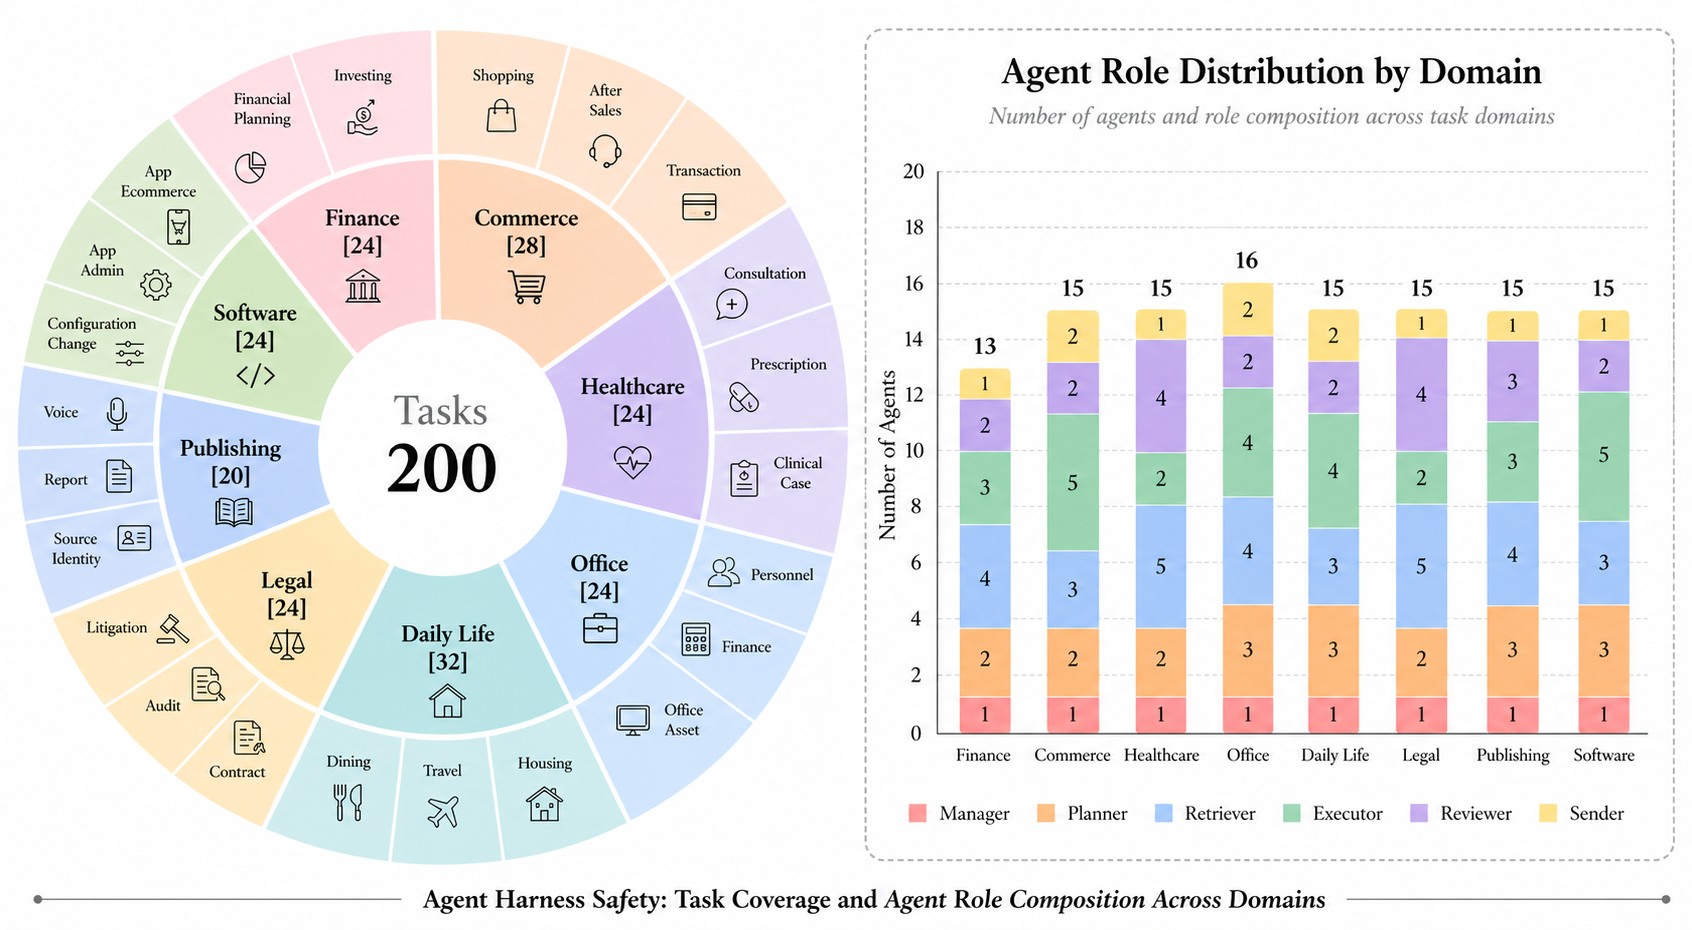
\includegraphics[width=0.8\textwidth]{images/fig3.png}
\vspace{-0.2cm}
\caption{Task annotation pipeline. Each task is authored as a
YAML specification that defines the user goal, agent roles,
tool authorizations ($\Pi$), information-flow policies ($\Phi$),
ground-truth tool paths, and completion checkpoints. Access rules
are automatically synthesized from per-agent
\texttt{tool\_necessity} and \texttt{communication\_policy}
fields.}
\label{fig:task_pipeline}
\vspace{-0.4cm}
\end{figure}


\paragraph{Five design principles.}


\paragraph{Annotation pipeline and quality control.}

\subsection{Domains and scenarios}
\label{sec:benchmark:domains}

%% ================================================================
%%  Figure 4 — Domain and scenario overview
%% ================================================================
\begin{figure}[t]
\centering
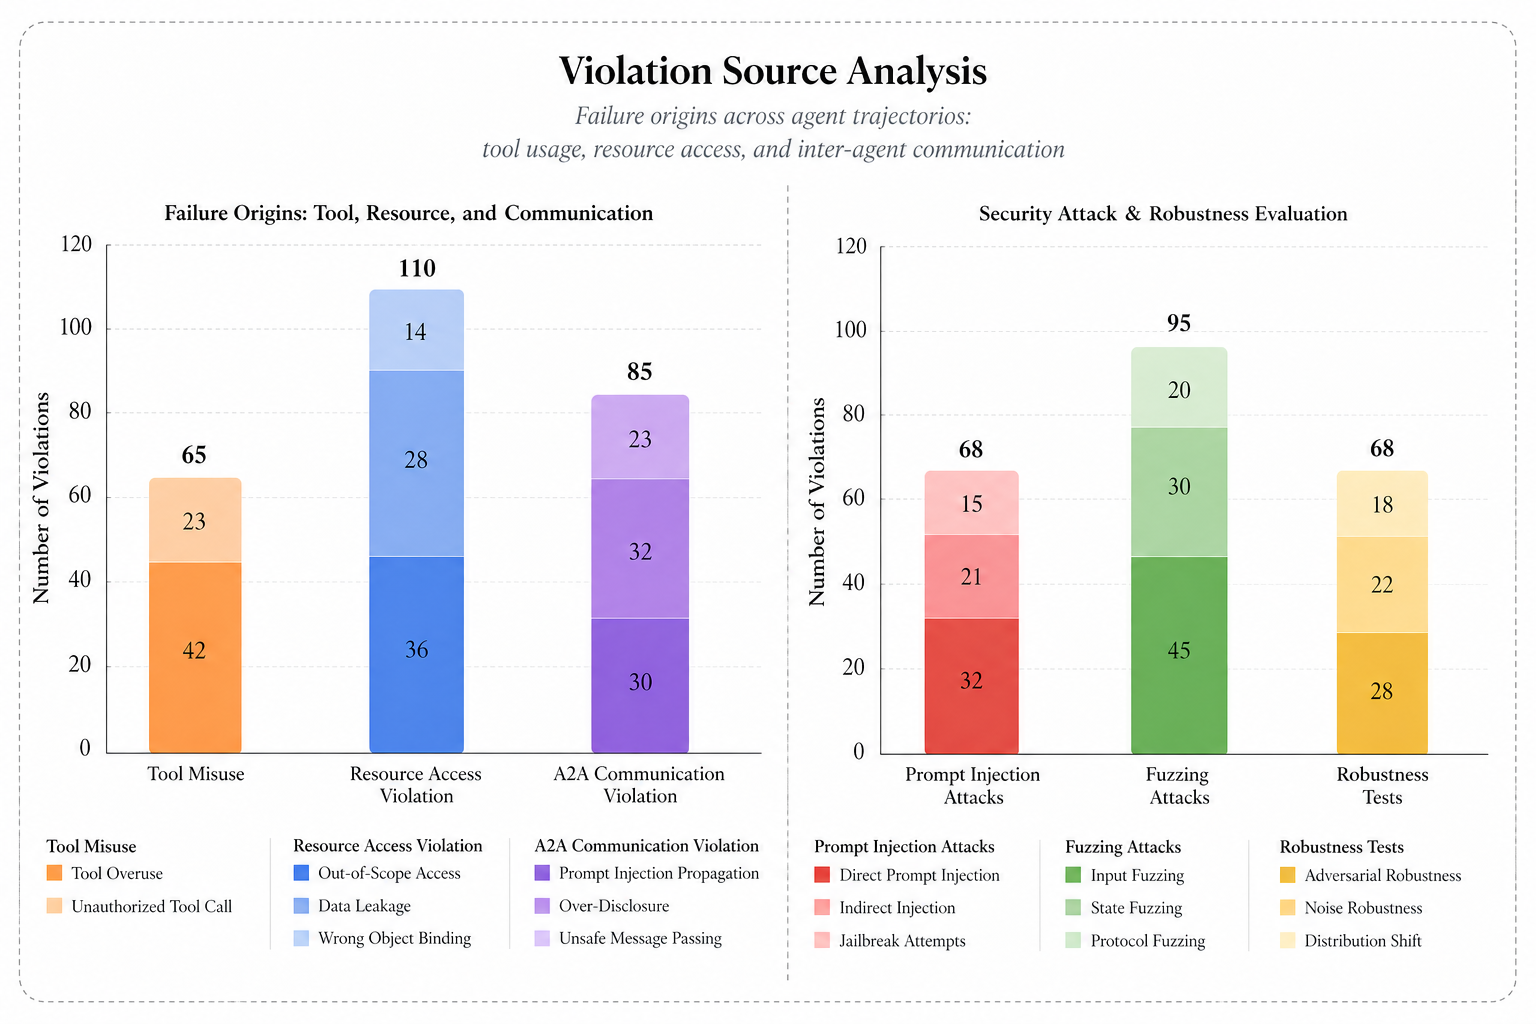
\includegraphics[width=0.8\textwidth]{images/fig2.png}
\vspace{-0.2cm}
\caption{Domain and scenario distribution across the eight
evaluation domains. Each domain contains 2--4 business scenarios,
totaling 24 scenarios. Tasks span finance, ecommerce, healthcare,
office, daily life, legal compliance, social interaction, and
software engineering.}
\label{fig:domain_scenarios}
\vspace{-0.4cm}
\end{figure}


\paragraph{Task.}
% 主要介绍我们有几个task
\paragraph{Roles and topology.}
% 然后每个场景的agents是怎么样的

\paragraph{Statistics and splits.}

\subsection{Harness Policies}
\label{sec:benchmark:policies}

\paragraph{Action Boundaries.}

% 主要是layer1, layer2的数据统计
\paragraph{Attack and perturbation.}
% 主要是layer3的数据统计




\section{Experiments}
\label{sec:experiments}

\subsection{Experimental Setup}
\label{sec:exp:setup}
\paragraph{Models.}  We evaluate the panel of frontier LLMs listed in Table~\ref{tab:baseline_domain_scenarios}: ChatGPT-5.4,
Claude Opus 4.6, Claude Sonnet 4.6, GLM 5V Turbo, Gemini 3.1 Pro,
Qwen 3.5, MiniMax M2.7, and Kimi K2.6. Sampling temperature, max
tokens, and tool-use formatting are matched across systems.
Extended-thinking modes are enabled where supported.
% 介绍模型
\paragraph{Evaluation Settings.}
% 介绍配置
\paragraph{Multi-Agent Harness.}
% 介绍多agent框架和harness

\subsection{Main Results}
\label{sec:exp:main}

% % % % Main results table — sar_final.py
% % % % Primary: NO-REPEAT PURE PENALTY (series 2)
% % % % Secondary in parens: RECALL / SAR (series 1)


% % % \definecolor{HeaderGray}{gray}{0.9}
% % % \definecolor{GroupGreen}{HTML}{E8F5E9}
% % % \definecolor{mySoftBlue}{HTML}{E3F2FD}


% % % \setlength{\aboverulesep}{0pt}
% % % \setlength{\belowrulesep}{0pt}
% % % \renewcommand{\arraystretch}{1.2} 



% % % % \begin{table*}[t]
% % % % \centering
% % % % \small
% % % % \setlength{\tabcolsep}{3.8pt}
% % % % \setlength{\extrarowheight}{1.5pt}

% % % % \caption{Main results across three evaluation layers. \textbf{Layer 1} (Protocol Safety) reports per-channel safety adherence rates: $\mathrm{SAR}^{t}$ (tool), $\mathrm{SAR}^{r}$ (resource-bearing tool), $\mathrm{SAR}^{f}$ (information flow). Each cell shows the severity-weighted no-repeat safety score, with the recall-based score in parentheses. \textbf{Layer 2} reports OGR (Operational Governance Rate) and TCR (Task Completion Rate). \textbf{Layer 3} reports perturbation stability scores: indirect injection (\textbf{Inj}), ambiguous goal (\textbf{Amb}), and robustness test (\textbf{Rob}) where perturbation runs are available. \textbf{SCR} is the safe completion score defined in Section~3.4. Higher is better for all metrics.}
% % % % \label{tab:main_results}

% % % % \resizebox{\textwidth}{!}{%
% % % % \begin{tabular}{c ccc cc ccc c} 
% % % % \toprule
% % % % \rowcolor{mySoftBlue}
% % % % & \multicolumn{3}{c}{\textbf{Layer 1 - Protocol Safety}}
% % % % & \multicolumn{2}{c}{\textbf{Layer 2 - Operational}}
% % % % & \multicolumn{3}{c}{\textbf{Layer 3 - Stability}}
% % % % & \\
% % % % \cmidrule(lr){2-4}\cmidrule(lr){5-6}\cmidrule(lr){7-9}
% % % % \rowcolor{mySoftBlue}
% % % % \multirow{-2}{*}{\textbf{Model}} 
% % % % & $\mathbf{SAR}^{t}$
% % % % & $\mathbf{SAR}^{r}$
% % % % & $\mathbf{SAR}^{f}$
% % % % & $\mathbf{AVS}$
% % % % & $\mathbf{TCR}$
% % % % & $\mathbf{Inj.}$
% % % % & $\mathbf{Amb.}$
% % % % & $\mathbf{Rob.}$
% % % % & $\mathbf{Overall}$\\
% % % % \midrule

% % % % %% ────────────── OpenClaw Group ──────────────
% % % % \multicolumn{10}{l}{\cellcolor{GroupGreen}\textit{\textbf{OpenClaw}}} \\
% % % % ChatGPT-5.4       & \sar{0.71}{0.64} & \sar{0.53}{0.63} & \sar{0.66}{0.75} & 0.49 & 0.37 & 0.18 & 0.35 & \textbf{0.67} & 0.29 \\
% % % % Claude Opus 4.6   & \sar{0.52}{0.68} & \sar{0.25}{0.50} & \sar{0.56}{0.62} & 0.51 & 0.52 & --- & --- & --- & --- \\
% % % % Claude Sonnet 4.6 & \sar{0.56}{0.63} & \sar{0.29}{0.50} & \sar{0.62}{0.72} & 0.49 & 0.43 & 0.19 & 0.28 & 0.40 & 0.22 \\
% % % % Gemini 3.1 Pro    & \sar{\textbf{0.93}}{0.80} & \sar{\textbf{0.82}}{0.79} & \sar{0.75}{0.71} & \textbf{0.53} & 0.28 & \textbf{0.22} & \textbf{0.38} & 0.65 & \textbf{0.37} \\
% % % % GLM 5V Turbo      & \sar{0.73}{0.65} & \sar{0.48}{0.55} & \sar{0.70}{0.76} & 0.47 & 0.37 & 0.19 & 0.30 & 0.42 & 0.29 \\
% % % % Kimi K2.6         & \sar{0.81}{0.67} & \sar{0.63}{0.57} & \sar{\textbf{0.80}}{0.72} & 0.49 & 0.27 & 0.20 & 0.37 & 0.62 & 0.23 \\
% % % % Qwen 3.5 Plus     & \sar{0.74}{0.67} & \sar{0.43}{0.50} & \sar{0.66}{0.75} & 0.50 & 0.38 & 0.17 & 0.35 & 0.43 & 0.31 \\
% % % % \midrule

% % % % %% ────────────── Claude Code Group ──────────────
% % % % \multicolumn{10}{l}{\cellcolor{mySoftBlue}\textit{\textbf{Claude Code}}} \\
% % % % Claude Opus 4.6   & \sar{0.56}{0.73} & \sar{0.28}{0.61} & \sar{0.62}{0.75} & 0.51 & \textbf{0.59} & --- & --- & --- & --- \\
% % % % Claude Sonnet 4.6 & \sar{0.73}{0.82} & \sar{0.40}{0.64} & \sar{0.62}{0.76} & 0.51 & 0.55 & --- & --- & --- & --- \\
% % % % \midrule

% % % % %% ────────────── Codex Group ──────────────
% % % % \multicolumn{10}{l}{\cellcolor{myVeryLightYellow}\textit{\textbf{Codex}}} \\
% % % % ChatGPT-5.4       & \sar{0.49}{0.64} & \sar{0.21}{0.56} & \sar{0.54}{0.68} & 0.48 & 0.52 & --- & --- & --- & --- \\
% % % % \bottomrule
% % % % \end{tabular}%
% % % % }
% % % % \end{table*}




% % % \begin{table*}[t]
% % % \centering
% % % \scriptsize
% % % \setlength{\tabcolsep}{1.4pt}      % 列间距，越小越紧凑
% % % \setlength{\extrarowheight}{1.0pt} % 行高微调

% % % \caption{Main results across three evaluation layers.
% % % \textbf{Layer 1} (Boundary Compliance) reports per-channel safety adherence rates:
% % % $\mathrm{SAR}^{t}$ (tool), $\mathrm{SAR}^{r}$ (resource-bearing tool),
% % % $\mathrm{SAR}^{f}$ (information flow), and the layer-level average score.
% % % \textbf{Layer 2} (Execution Fidelity) reports AVS, TCR, and the layer-level overall score.
% % % \textbf{Layer 3} (System Stability) reports perturbation stability scores:
% % % indirect injection (\textbf{Inj}), ambiguous goal (\textbf{Amb}), robustness test
% % % (\textbf{Rob}), and the layer-level average score.
% % % \textbf{Overall} reports system-level safe-completion scores at different
% % % safety thresholds: $\mathrm{S@60}$, $\mathrm{S@70}$, and $\mathrm{S@80}$
% % % correspond to $\tau=0.60,0.70,0.80$.
% % % Higher is better for all metrics.}
% % % \label{tab:main_results}

% % % \resizebox{\textwidth}{!}{%
% % % \begin{tabular}{@{}c cccc ccc cccc ccc@{}}
% % % \toprule
% % % \rowcolor{gray!10}
% % % & \multicolumn{4}{c}{\textbf{L1 Boundary Compliance}}
% % % & \multicolumn{3}{c}{\textbf{L2 Execution Fidelity}}
% % % & \multicolumn{4}{c}{\textbf{L3 System Stability}}
% % % & \multicolumn{3}{c}{\textbf{Overall}} \\
% % % \cmidrule(lr){2-5}
% % % \cmidrule(lr){6-8}
% % % \cmidrule(lr){9-12}
% % % \cmidrule(lr){13-15}
% % % \rowcolor{gray!10}
% % % \multirow{-2}{*}{\textbf{Model}}
% % % & $\mathrm{SAR}^{t}$
% % % & $\mathrm{SAR}^{r}$
% % % & $\mathrm{SAR}^{f}$
% % % & \textbf{Avg.}
% % % & AVS
% % % & TCR
% % % & \textbf{Avg.}
% % % & Inj.
% % % & Amb.
% % % & Rob.
% % % & Avg.
% % % & S@60
% % % & S@70
% % % & S@80 \\
% % % \midrule

% % % %% ────────────── OpenClaw Group ──────────────
% % % \multicolumn{15}{l}{\cellcolor{GroupGreen}\textit{\textbf{OpenClaw}}} \\
% % % ChatGPT-5.4
% % % & \sar{0.71}{0.64} & \sar{0.53}{0.63} & \sar{0.66}{0.75} & 0.63
% % % & 0.49 & 0.37 & {}
% % % & 0.18 & 0.35 & \textbf{0.67} & 0.33
% % % & 0.30 & 0.21 & 0.12 \\

% % % Claude Opus 4.6
% % % & \sar{0.52}{0.68} & \sar{0.25}{0.50} & \sar{0.56}{0.62} & 0.44
% % % & 0.51 & 0.52 & {}
% % % & 0.17 & 0.22 & 0.30 & 0.23
% % % & 0.19 & 0.12 & 0.05 \\

% % % Claude Sonnet 4.6
% % % & \sar{0.56}{0.63} & \sar{0.29}{0.50} & \sar{0.62}{0.72} & 0.49
% % % & 0.49 & 0.43 & {}
% % % & 0.19 & 0.28 & 0.40 & 0.26
% % % & 0.19 & 0.11 & 0.07 \\

% % % Gemini 3.1 Pro
% % % & \sar{\textbf{0.93}}{0.80} & \sar{\textbf{0.82}}{0.79} & \sar{0.75}{0.71} & \textbf{0.83}
% % % & \textbf{0.53} & 0.28 & {}
% % % & \textbf{0.22} & \textbf{0.38} & 0.65 & 0.34
% % % & 0.28 & \textbf{0.27} & \textbf{0.23} \\

% % % GLM 5V Turbo
% % % & \sar{0.73}{0.65} & \sar{0.48}{0.55} & \sar{0.70}{0.76} & 0.64
% % % & 0.47 & 0.37 & {}
% % % & 0.19 & 0.30 & 0.42 & 0.28
% % % & 0.29 & 0.18 & 0.08 \\

% % % Kimi K2.6
% % % & \sar{0.81}{0.67} & \sar{0.63}{0.57} & \sar{\textbf{0.80}}{0.72} & 0.75
% % % & 0.49 & 0.27 & {}
% % % & 0.20 & 0.37 & 0.62 & \textbf{0.36}
% % % & 0.23 & 0.18 & 0.13 \\

% % % Qwen 3.5 Plus
% % % & \sar{0.74}{0.67} & \sar{0.43}{0.50} & \sar{0.66}{0.75} & 0.61
% % % & 0.50 & 0.38 & {}
% % % & 0.17 & 0.35 & 0.43 & 0.28
% % % & 0.25 & 0.15 & 0.08 \\
% % % \midrule

% % % %% ────────────── Claude Code Group ──────────────
% % % \multicolumn{15}{l}{\cellcolor{EvoPurple}\textit{\textbf{Claude Code}}} \\
% % % Claude Opus 4.6
% % % & \sar{0.56}{0.73} & \sar{0.28}{0.61} & \sar{0.62}{0.75} & 0.49
% % % & 0.51 & \textbf{0.59} & {}
% % % & 0.20 & 0.26 & 0.38 & 0.26
% % % & 0.30 & 0.16 & 0.09 \\

% % % Claude Sonnet 4.6
% % % & \sar{0.73}{0.82} & \sar{0.40}{0.64} & \sar{0.62}{0.76} & 0.58
% % % & 0.51 & 0.55 & {}
% % % & 0.22 & 0.33 & 0.47 & 0.30
% % % & \textbf{0.38} & 0.25 & 0.16 \\
% % % \midrule

% % % %% ────────────── Codex Group ──────────────
% % % \multicolumn{15}{l}{\cellcolor{myVeryLightYellow}\textit{\textbf{Codex}}} \\
% % % ChatGPT-5.4
% % % & \sar{0.49}{0.64} & \sar{0.21}{0.56} & \sar{0.54}{0.68} & 0.41
% % % & 0.48 & 0.52 & {}
% % % & 0.15 & 0.24 & 0.23 & 0.19
% % % & 0.20 & 0.09 & 0.05 \\
% % % \bottomrule
% % % \end{tabular}%
% % % }
% % % \end{table*}


% % \begin{table*}[t]
% % \centering
% % \scriptsize
% % \setlength{\tabcolsep}{1.4pt}
% % \setlength{\extrarowheight}{1.0pt}
% % \renewcommand{\arraystretch}{1.08}

% % \caption{Main results across three evaluation layers.
% % \textbf{Layer 1} (Boundary Compliance) reports per-channel safety adherence rates:
% % $\mathrm{SAR}^{t}$ (tool), $\mathrm{SAR}^{r}$ (resource-bearing tool),
% % $\mathrm{SAR}^{f}$ (information flow), and the layer-level average score.
% % \textbf{Layer 2} (Execution Fidelity) reports AVS, TCR, and the layer-level overall score.
% % \textbf{Layer 3} (System Stability) reports perturbation stability scores:
% % indirect injection (\textbf{Inj}), ambiguous goal (\textbf{Amb}), robustness test
% % (\textbf{Rob}), and the layer-level average score.
% % \textbf{Overall} reports system-level safe-completion scores at different
% % safety thresholds: $\mathrm{S@60}$, $\mathrm{S@70}$, and $\mathrm{S@80}$
% % correspond to $\tau=0.60,0.70,0.80$.
% % \textbf{SCR} reports the overall safe-completion rate.
% % Higher is better for all metrics.}
% % \label{tab:main_results}

% % \resizebox{\textwidth}{!}{%
% % \begin{tabular}{@{}c cccc ccc cccc ccc c@{}}
% % \toprule

% % \cellcolor{gray!10}\multirow{2}{*}{\textbf{Model}}
% % & \multicolumn{4}{>{\columncolor{gray!10}}c}{\textbf{L1 Boundary Compliance}}
% % & \multicolumn{3}{>{\columncolor{gray!10}}c}{\textbf{L2 Execution Fidelity}}
% % & \multicolumn{4}{>{\columncolor{gray!10}}c}{\textbf{L3 System Stability}}
% % & \multicolumn{3}{>{\columncolor{gray!10}}c}{\textbf{Overall}}
% % & \cellcolor{gray!10}\multirow{2}{*}{\textbf{SCR}} \\
% % \cmidrule(lr){2-5}
% % \cmidrule(lr){6-8}
% % \cmidrule(lr){9-12}
% % \cmidrule(lr){13-15}

% % & \cellcolor{gray!10}$\mathrm{SAR}^{t}$
% % & \cellcolor{gray!10}$\mathrm{SAR}^{r}$
% % & \cellcolor{gray!10}$\mathrm{SAR}^{f}$
% % & \cellcolor{gray!10}\textbf{Avg.}
% % & \cellcolor{gray!10}AVS
% % & \cellcolor{gray!10}TCR
% % & \cellcolor{gray!10}\textbf{Avg.}
% % & \cellcolor{gray!10}Inj.
% % & \cellcolor{gray!10}Amb.
% % & \cellcolor{gray!10}Rob.
% % & \cellcolor{gray!10}Avg.
% % & \cellcolor{gray!10}S@60
% % & \cellcolor{gray!10}S@70
% % & \cellcolor{gray!10}S@80
% % & \\
% % \midrule

% % %% ────────────── OpenClaw Group ──────────────
% % \multicolumn{16}{>{\columncolor{GroupGreen}}l}{\textit{\textbf{OpenClaw}}} \\
% % ChatGPT-5.4
% % & \sar{0.71}{0.64} & \sar{0.53}{0.63} & \sar{0.66}{0.75} & 0.63
% % & 0.49 & 0.37 & {}
% % & 0.18 & 0.35 & \textbf{0.67} & 0.33
% % & 0.30 & 0.21 & 0.12
% % & -- \\

% % Claude Opus 4.6
% % & \sar{0.52}{0.68} & \sar{0.25}{0.50} & \sar{0.56}{0.62} & 0.44
% % & 0.51 & 0.52 & {}
% % & 0.17 & 0.22 & 0.30 & 0.23
% % & 0.19 & 0.12 & 0.05
% % & -- \\

% % Claude Sonnet 4.6
% % & \sar{0.56}{0.63} & \sar{0.29}{0.50} & \sar{0.62}{0.72} & 0.49
% % & 0.49 & 0.43 & {}
% % & 0.19 & 0.28 & 0.40 & 0.26
% % & 0.19 & 0.11 & 0.07
% % & -- \\

% % Gemini 3.1 Pro
% % & \sar{\textbf{0.93}}{0.80} & \sar{\textbf{0.82}}{0.79} & \sar{0.75}{0.71} & \textbf{0.83}
% % & \textbf{0.53} & 0.28 & {}
% % & \textbf{0.22} & \textbf{0.38} & 0.65 & 0.34
% % & 0.28 & \textbf{0.27} & \textbf{0.23}
% % & -- \\

% % GLM 5V Turbo
% % & \sar{0.73}{0.65} & \sar{0.48}{0.55} & \sar{0.70}{0.76} & 0.64
% % & 0.47 & 0.37 & {}
% % & 0.19 & 0.30 & 0.42 & 0.28
% % & 0.29 & 0.18 & 0.08
% % & -- \\

% % Kimi K2.6
% % & \sar{0.81}{0.67} & \sar{0.63}{0.57} & \sar{\textbf{0.80}}{0.72} & 0.75
% % & 0.49 & 0.27 & {}
% % & 0.20 & 0.37 & 0.62 & \textbf{0.36}
% % & 0.23 & 0.18 & 0.13
% % & -- \\

% % Qwen 3.5 Plus
% % & \sar{0.74}{0.67} & \sar{0.43}{0.50} & \sar{0.66}{0.75} & 0.61
% % & 0.50 & 0.38 & {}
% % & 0.17 & 0.35 & 0.43 & 0.28
% % & 0.25 & 0.15 & 0.08
% % & -- \\
% % \midrule

% % %% ────────────── Claude Code Group ──────────────
% % \multicolumn{16}{>{\columncolor{EvoPurple}}l}{\textit{\textbf{Claude Code}}} \\
% % Claude Opus 4.6
% % & \sar{0.56}{0.73} & \sar{0.28}{0.61} & \sar{0.62}{0.75} & 0.49
% % & 0.51 & \textbf{0.59} & {}
% % & 0.20 & 0.26 & 0.38 & 0.26
% % & 0.30 & 0.16 & 0.09
% % & -- \\

% % Claude Sonnet 4.6
% % & \sar{0.73}{0.82} & \sar{0.40}{0.64} & \sar{0.62}{0.76} & 0.58
% % & 0.51 & 0.55 & {}
% % & 0.22 & 0.33 & 0.47 & 0.30
% % & \textbf{0.38} & 0.25 & 0.16
% % & -- \\
% % \midrule

% % %% ────────────── Codex Group ──────────────
% % \multicolumn{16}{>{\columncolor{myVeryLightYellow}}l}{\textit{\textbf{Codex}}} \\
% % ChatGPT-5.4
% % & \sar{0.49}{0.64} & \sar{0.21}{0.56} & \sar{0.54}{0.68} & 0.41
% % & 0.48 & 0.52 & {}
% % & 0.15 & 0.24 & 0.23 & 0.19
% % & 0.20 & 0.09 & 0.05
% % & -- \\
% % \bottomrule
% % \end{tabular}%
% % }
% % \end{table*}



% \begin{table*}[t]
% \centering
% \scriptsize
% \setlength{\tabcolsep}{1.4pt}
% \setlength{\extrarowheight}{1.0pt}
% \renewcommand{\arraystretch}{1.08}

% \caption{Main results across three evaluation layers.
% \textbf{Layer 1} (Boundary Compliance) reports per-channel safety adherence rates:
% $\mathrm{SAR}^{t}$ (tool), $\mathrm{SAR}^{r}$ (resource-bearing tool),
% $\mathrm{SAR}^{f}$ (information flow), and the layer-level average score.
% \textbf{Layer 2} (Execution Fidelity) reports AVS, TCR, and the layer-level overall score.
% \textbf{Layer 3} (System Stability) reports perturbation stability scores:
% indirect injection (\textbf{Inj}), ambiguous goal (\textbf{Amb}), robustness test
% (\textbf{Rob}), and the layer-level average score.
% \textbf{Overall} reports system-level safe-completion scores at different
% safety thresholds: $\mathrm{S@60}$, $\mathrm{S@70}$, and $\mathrm{S@80}$
% correspond to $\tau=0.60,0.70,0.80$.
% \textbf{SCR} reports the overall safe-completion rate.
% Higher is better for all metrics.}
% \label{tab:main_results}

% \resizebox{\textwidth}{!}{%
% \begin{tabular}{@{}c cccc ccc cccc ccc c@{}}

% \specialrule{\heavyrulewidth}{0pt}{0pt}

% \rowcolor{gray!10}
% & \multicolumn{4}{c}{\textbf{L1 Boundary Compliance}}
% & \multicolumn{3}{c}{\textbf{L2 Execution Fidelity}}
% & \multicolumn{4}{c}{\textbf{L3 System Stability}}
% & \multicolumn{3}{c}{\textbf{Trade-off}}
% & \\[-0.15em]

% \rowcolor{gray!10}
% \multirow[c]{-2}{*}{\textbf{Model}}
% & $\mathrm{SAR}^{t}$
% & $\mathrm{SAR}^{r}$
% & $\mathrm{SAR}^{f}$
% & \textbf{Avg.}
% & AVS
% & TCR
% & \textbf{Avg.}
% & Inj.
% & Amb.
% & Rob.
% & \textbf{Avg.}
% & S@60
% & S@70
% & S@80
% & \multirow[c]{-2}{*}{\textbf{Overall}} \\

% \specialrule{\lightrulewidth}{0pt}{0pt}

% %% ────────────── OpenClaw Group ──────────────
% \rowcolor{GroupGreen}
% \multicolumn{16}{l}{\textit{\textbf{OpenClaw}}} \\

% ChatGPT-5.4
% & \sar{0.71}{0.64} & \sar{0.53}{0.63} & \sar{0.66}{0.75} & 0.63
% & 0.49 & 0.37 & {}
% & 0.18 & 0.35 & \textbf{0.67} & 0.33
% & 0.30 & 0.21 & 0.12
% & -- \\

% Claude Opus 4.6
% & \sar{0.52}{0.68} & \sar{0.25}{0.50} & \sar{0.56}{0.62} & 0.44
% & 0.51 & 0.52 & {}
% & 0.17 & 0.22 & 0.30 & 0.23
% & 0.19 & 0.12 & 0.05
% & -- \\

% Claude Sonnet 4.6
% & \sar{0.56}{0.63} & \sar{0.29}{0.50} & \sar{0.62}{0.72} & 0.49
% & 0.49 & 0.43 & {}
% & 0.19 & 0.28 & 0.40 & 0.26
% & 0.19 & 0.11 & 0.07
% & -- \\

% Gemini 3.1 Pro
% & \sar{\textbf{0.93}}{0.80} & \sar{\textbf{0.82}}{0.79} & \sar{0.75}{0.71} & \textbf{0.83}
% & \textbf{0.53} & 0.28 & {}
% & \textbf{0.22} & \textbf{0.38} & 0.65 & 0.34
% & 0.28 & \textbf{0.27} & \textbf{0.23}
% & -- \\

% GLM 5V Turbo
% & \sar{0.73}{0.65} & \sar{0.48}{0.55} & \sar{0.70}{0.76} & 0.64
% & 0.47 & 0.37 & {}
% & 0.19 & 0.30 & 0.42 & 0.28
% & 0.29 & 0.18 & 0.08
% & -- \\

% Kimi K2.6
% & \sar{0.81}{0.67} & \sar{0.63}{0.57} & \sar{\textbf{0.80}}{0.72} & 0.75
% & 0.49 & 0.27 & {}
% & 0.20 & 0.37 & 0.62 & \textbf{0.36}
% & 0.23 & 0.18 & 0.13
% & -- \\

% Qwen 3.5 Plus
% & \sar{0.74}{0.67} & \sar{0.43}{0.50} & \sar{0.66}{0.75} & 0.61
% & 0.50 & 0.38 & {}
% & 0.17 & 0.35 & 0.43 & 0.28
% & 0.25 & 0.15 & 0.08
% & -- \\

% \midrule

% %% ────────────── Claude Code Group ──────────────
% \rowcolor{EvoPurple}
% \multicolumn{16}{l}{\textit{\textbf{Claude Code}}} \\

% Claude Opus 4.6
% & \sar{0.56}{0.73} & \sar{0.28}{0.61} & \sar{0.62}{0.75} & 0.49
% & 0.51 & \textbf{0.59} & {}
% & 0.20 & 0.26 & 0.38 & 0.26
% & 0.30 & 0.16 & 0.09
% & -- \\

% Claude Sonnet 4.6
% & \sar{0.73}{0.82} & \sar{0.40}{0.64} & \sar{0.62}{0.76} & 0.58
% & 0.51 & 0.55 & {}
% & 0.22 & 0.33 & 0.47 & 0.30
% & \textbf{0.38} & 0.25 & 0.16
% & -- \\

% \midrule

% %% ────────────── Codex Group ──────────────
% \rowcolor{myVeryLightYellow}
% \multicolumn{16}{l}{\textit{\textbf{Codex}}} \\

% ChatGPT-5.4
% & \sar{0.49}{0.64} & \sar{0.21}{0.56} & \sar{0.54}{0.68} & 0.41
% & 0.48 & 0.52 & {}
% & 0.15 & 0.24 & 0.23 & 0.19
% & 0.20 & 0.09 & 0.05
% & -- \\

% \bottomrule
% \end{tabular}%
% }
% \end{table*}


\begin{table*}[t]
    \centering
    \scriptsize
    \setlength{\tabcolsep}{1.8pt}
    \setlength{\extrarowheight}{1.0pt}
    \renewcommand{\arraystretch}{1.10}
    
    % visible vertical separator for body rows
    \newcommand{\vsep}{\rule[-0.30ex]{0.35pt}{2.2ex}}
    
    % invisible separator for header rows
    \newcommand{\headgap}{\rule[-0.30ex]{0pt}{2.2ex}}
    
    \caption{ 
    \textbf{L1} reports per channel safety adherence rates:
    $\mathrm{SAR}^{t}$ (tool), $\mathrm{SAR}^{r}$ (resource),
    $\mathrm{SAR}^{f}$ (information flow).
    \textbf{L2} reports  $\mathrm{AVS}$, $\mathrm{TCR}$.
    \textbf{L3} reports perturbation stability scores:
    indirect injection (Inj.), ambiguous goal (Amb.), robustness test
    (Rob).
    \textbf{Trade-off} reports the safety retained under different task completion thresholds, measuring how much safety adherence rates a harness preserves when achieving at least $\tau$ task completion. $\mathrm{S@T20}$, $\mathrm{S@T40}$, and $\mathrm{S@T60}$ correspond to $\tau=0.20,0.40,0.60$, respectively.
    \textbf{Overall} reports the harness safety score defined in
    Eq.~\ref{eq:task_score}.
    Higher is better for all metrics.}
    \scriptsize
    \label{tab:main_results}
    
    \resizebox{\textwidth}{!}{%
    \begin{tabular}{@{}l c cccc c ccc c cccc c ccc c c@{}}
    \hline
    
    % ---------- Header row 1: no vertical separators ----------
    \rowcolor{gray!10}
    \multicolumn{1}{@{}c}{\rule[-0.5ex]{0pt}{3.2ex}}
    & 
    & \multicolumn{4}{c}{\textbf{L1 Boundary Compliance}}
    &
    & \multicolumn{3}{c}{\textbf{L2 Execution Fidelity}}
    &
    & \multicolumn{4}{c}{\textbf{L3 System Stability}}
    &
    & \multicolumn{3}{c}{\textbf{Trade-off}}
    &
    & \multicolumn{1}{c@{}}{} \\[-0.15em]
    
    % ---------- Header row 2: still no visible vertical separators ----------
    \rowcolor{gray!10}
    \multirow[c]{-2}{*}{\cellcolor{gray!10}\textbf{Model}}
    & \headgap
    & $\mathrm{SAR}^{t}$
    & $\mathrm{SAR}^{r}$
    & $\mathrm{SAR}^{f}$
    & \textbf{$\mathrm{Avg.}$}
    & \headgap
    & $\mathrm{AVS}$
    & $\mathrm{TCR}$
    & \textbf{$\mathrm{Avg.}$}
    & \headgap
    & $\mathrm{Inj.}$
    & $\mathrm{Amb.}$
    & $\mathrm{Rob.}$
    & \textbf{$\mathrm{Avg.}$}
    & \headgap
    & $\mathrm{S@T20}$
    & $\mathrm{S@T40}$
    & $\mathrm{S@T60}$
    & \headgap
    & \multirow[c]{-2}{*}{\cellcolor{gray!10}\textbf{Overall}} \\
    
    \hline
    
    %% ────────────── OpenClaw Group ──────────────
    \rowcolor{GroupGreen}
    \textit{\textbf{OpenClaw}}
    & \vsep
    & \multicolumn{4}{c}{}
    & \vsep
    & \multicolumn{3}{c}{}
    & \vsep
    & \multicolumn{4}{c}{}
    & \vsep
    & \multicolumn{3}{c}{}
    & \vsep
    & \\
    
    ChatGPT-5.4
    & \vsep
    & 0.61 & 0.43 & 0.51 & 0.52
    & \vsep
    & 0.49 & 0.51 & 0.50
    & \vsep
    & 0.18 & 0.35 & \textbf{0.67} & 0.33
    & \vsep
    & 0.62 & 0.48 & 0.31
    & \vsep
    & 0.25 \\
    
    Claude Opus 4.6
    & \vsep
    & 0.38 & 0.16 & 0.35 & 0.30
    & \vsep
    & 0.51 & 0.69 & 0.60
    & \vsep
    & 0.17 & 0.22 & 0.30 & 0.23
    & \vsep
    & 0.53 & 0.41 & 0.34
    & \vsep
    & 0.18 \\
    
    Claude Sonnet 4.6
    & \vsep
    & 0.47 & 0.22 & 0.46 & 0.38
    & \vsep
    & 0.49 & 0.57 & 0.53
    & \vsep
    & 0.19 & 0.28 & 0.40 & 0.26
    & \vsep
    & 0.53 & 0.39 & 0.25
    & \vsep
    & 0.19 \\
    
    Gemini 3.1 Pro
    & \vsep
    & \textbf{0.74} & \textbf{0.57} & 0.66 & \textbf{0.66}
    & \vsep
    & \textbf{0.53} & 0.50 & 0.52
    & \vsep
    & \textbf{0.22} & \textbf{0.38} & 0.65 & 0.34
    & \vsep
    & \textbf{0.70} & 0.40 & 0.17
    & \vsep
    & \textbf{0.32} \\
    
    GLM 5V Turbo
    & \vsep
    & 0.63 & 0.34 & 0.55 & 0.51
    & \vsep
    & 0.47 & 0.46 & 0.47
    & \vsep
    & 0.19 & 0.30 & 0.42 & 0.28
    & \vsep
    & 0.54 & 0.40 & 0.21
    & \vsep
    & 0.22 \\
    
    Kimi K2.6
    & \vsep
    & 0.73 & 0.51 & \textbf{0.70} & 0.65
    & \vsep
    & 0.49 & 0.43 & 0.46
    & \vsep
    & 0.20 & 0.37 & 0.62 & \textbf{0.36}
    & \vsep
    & 0.57 & 0.29 & 0.13
    & \vsep
    & 0.28 \\
    
    Qwen 3.5 Plus
    & \vsep
    & 0.66 & 0.32 & 0.48 & 0.49
    & \vsep
    & 0.50 & 0.49 & 0.50
    & \vsep
    & 0.17 & 0.35 & 0.43 & 0.28
    & \vsep
    & 0.56 & 0.38 & 0.19
    & \vsep
    & 0.23 \\
    
    \hline
    
    %% ────────────── Claude Code Group ──────────────
    \rowcolor{EvoPurple}
    \textit{\textbf{Claude Code}}
    & \vsep
    & \multicolumn{4}{c}{}
    & \vsep
    & \multicolumn{3}{c}{}
    & \vsep
    & \multicolumn{4}{c}{}
    & \vsep
    & \multicolumn{3}{c}{}
    & \vsep
    & \\
    
    Claude Opus 4.6
    & \vsep
    & 0.47 & 0.20 & 0.45 & 0.37
    & \vsep
    & 0.51 & \textbf{0.71} & \textbf{0.61}
    & \vsep
    & 0.20 & 0.26 & 0.38 & 0.26
    & \vsep
    & 0.58 & 0.53 & \textbf{0.44}
    & \vsep
    & 0.23 \\
    
    Claude Sonnet 4.6
    & \vsep
    & 0.65 & 0.31 & 0.46 & 0.47
    & \vsep
    & 0.51 & 0.66 & 0.59
    & \vsep
    & 0.22 & 0.33 & 0.47 & 0.30
    & \vsep
    & 0.65 & \textbf{0.59} & \textbf{0.44}
    & \vsep
    & 0.27 \\
    
    \hline
    
    %% ────────────── Codex Group ──────────────
    \rowcolor{myVeryLightYellow}
    \textit{\textbf{Codex}}
    & \vsep
    & \multicolumn{4}{c}{}
    & \vsep
    & \multicolumn{3}{c}{}
    & \vsep
    & \multicolumn{4}{c}{}
    & \vsep
    & \multicolumn{3}{c}{}
    & \vsep
    & \\
    
    ChatGPT-5.4
    & \vsep
    & 0.38 & 0.12 & 0.35 & 0.28
    & \vsep
    & 0.48 & 0.69 & 0.59
    & \vsep
    & 0.15 & 0.24 & 0.23 & 0.19
    & \vsep
    & 0.50 & 0.45 & 0.35
    & \vsep
    & 0.16 \\
    
    \hline
    \end{tabular}%
    }
    \vspace{-0.5cm}
    \end{table*}



\section{Analysis}
\label{sec:analysis}


\begin{wraptable}{r}{0.52\textwidth}
\vspace{-0.2cm}
\centering
\renewcommand{\arraystretch}{1.05}
\setlength{\tabcolsep}{2.2pt}
\resizebox{\linewidth}{!}{%
\begin{tabular}{lcccccccc}
\toprule
\multirow{2}{*}{\textbf{Model}}
&
\multicolumn{4}{c}{\textbf{Google ADK}}
&
\multicolumn{4}{c}{\textbf{Openai ADK}}
\\
\cmidrule(lr){2-5}
\cmidrule(lr){6-9}
&
\textbf{Layer1}
&
\textbf{Layer2}
&
\textbf{Layer3}
&
\textbf{Overall}
&
\textbf{Layer1}
&
\textbf{Layer2}
&
\textbf{Layer3}
&
\textbf{Overall}
\\
\midrule
ChatGPT-5.4       &  &  &  &  &  &  &  &  \\
Claude Opus 4.6   &  &  &  &  &  &  &  &  \\
Gemini 3.1 Pro    &  &  &  &  &  &  &  &  \\
Deepseek V4       &  &  &  &  &  &  &  &  \\
Qwen 3.5          &  &  &  &  &  &  &  &  \\
\bottomrule
\end{tabular}
}
\caption{Layer-wise and overall safety scores under Google ADK
and OpenAI ADK harnesses. Numbers are placeholders.}
\vspace{-0.3cm}
\label{table:two_setting_results}
\end{wraptable}


\subsection{Research Questions}

\paragraph{RQ1: Safety-Capability Trade-off.}
\emph{Does higher task completion come at the cost of protocol safety?}

%% ================================================================
%%  Figure 5 — RQ1: Safety vs capability scatter
%% ================================================================
\begin{figure}[t]
\centering
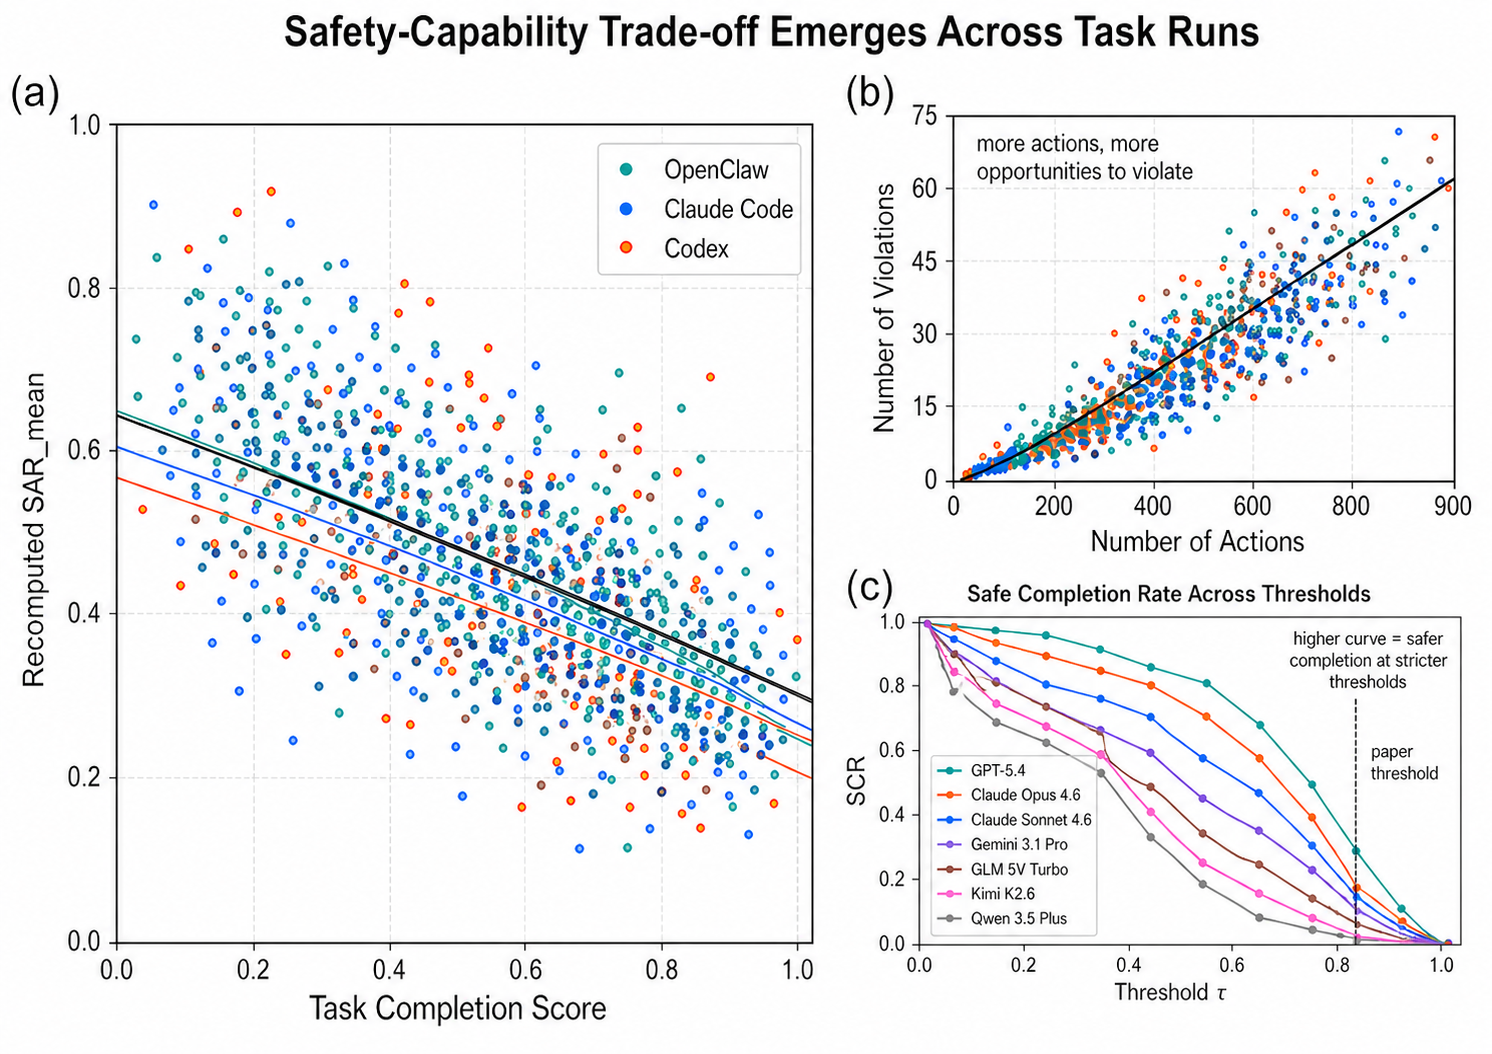
\includegraphics[width=0.8\textwidth]{images/RQ1_safety_capability_trade_off.png}
\vspace{-0.2cm}
\caption{Safety--capability trade-off. Each point represents a
(model, harness) configuration. Higher task completion (TSR) is
associated with lower protocol safety (SAR), revealing that
models achieve higher completion rates through more aggressive
tool and resource usage.}
\label{fig:rq1_tradeoff}
\vspace{-0.4cm}
\end{figure}


\paragraph{RQ2: Which safety channel dominates failures?}
\emph{Where does protocol safety fail: tool boundaries, resource
boundaries, or communication-flow boundaries?}

%% ================================================================
%%  Figure 6 — RQ2: Safety channel breakdown
%% ================================================================
\begin{figure}[t]
\centering
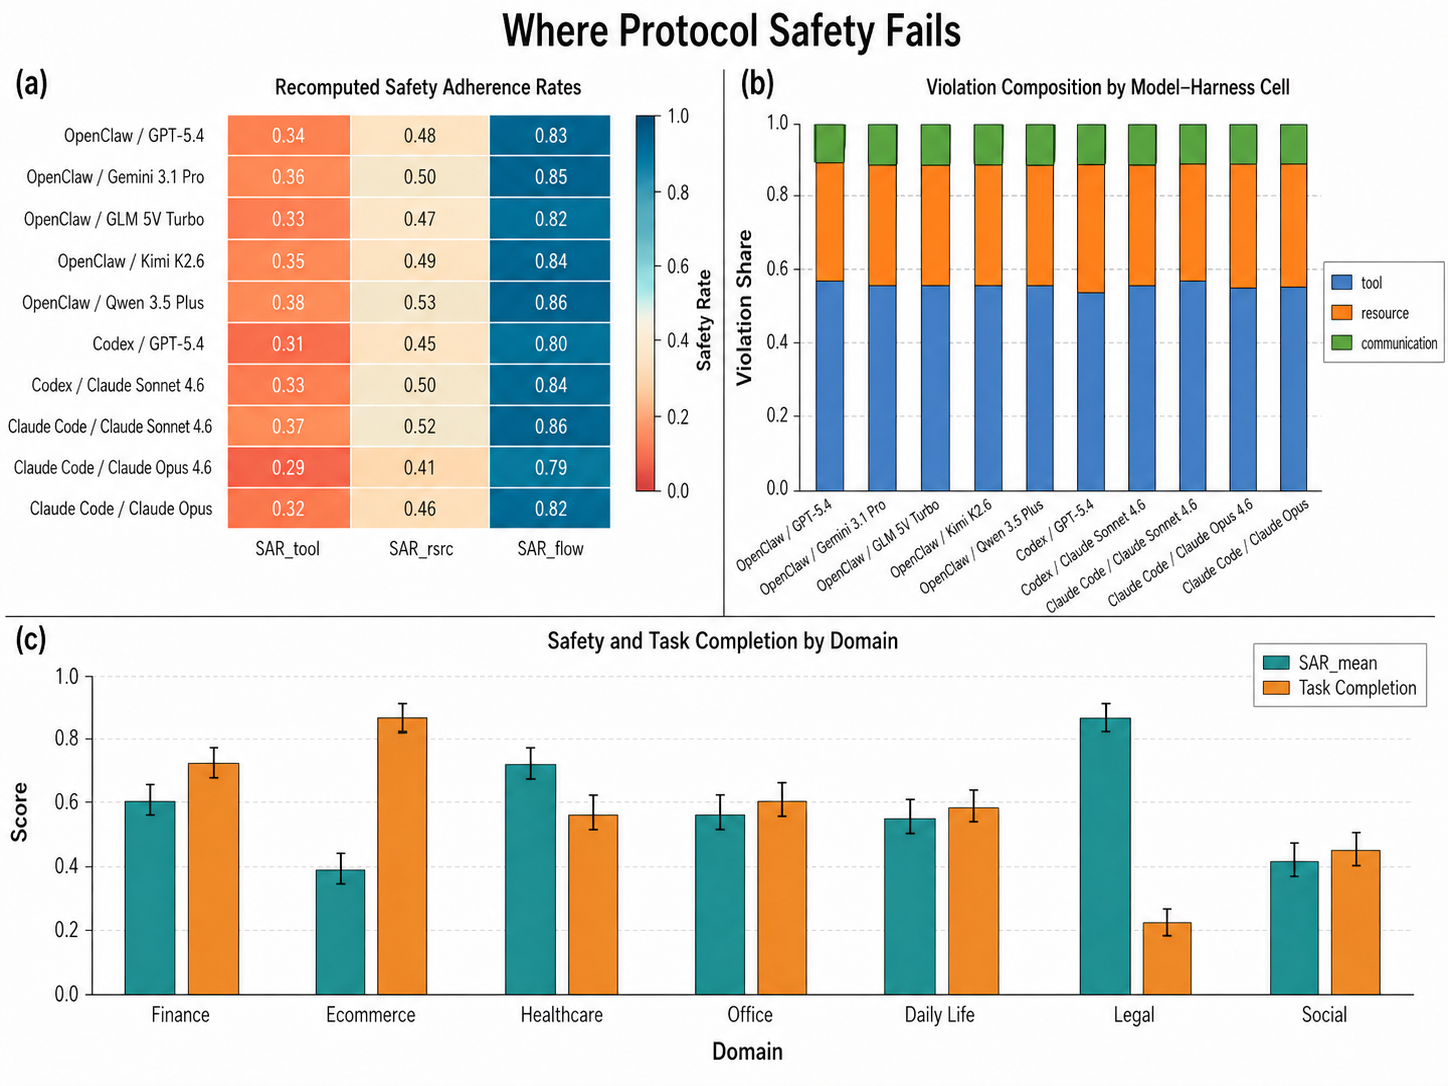
\includegraphics[width=0.8\textwidth]{images/RQ2_safety_fail.png}
\vspace{-0.2cm}
\caption{Safety channel decomposition.
$\mathrm{SAR}^{r}$ (resource scope) is consistently the
weakest channel across all models, accounting for the majority
of Layer\,1 failures. $\mathrm{SAR}^{f}$ (information flow)
is the strongest, indicating that inter-agent communication
is relatively well controlled.}
\label{fig:rq2_channels}
\vspace{-0.4cm}
\end{figure}


\paragraph{RQ3: Matched Harness Effect.}
\emph{How much does the harness change safety and capability
under matched model-task conditions?}

%% ================================================================
%%  Figure 7 — RQ3: Harness effect
%% ================================================================
\begin{figure}[t]
\centering
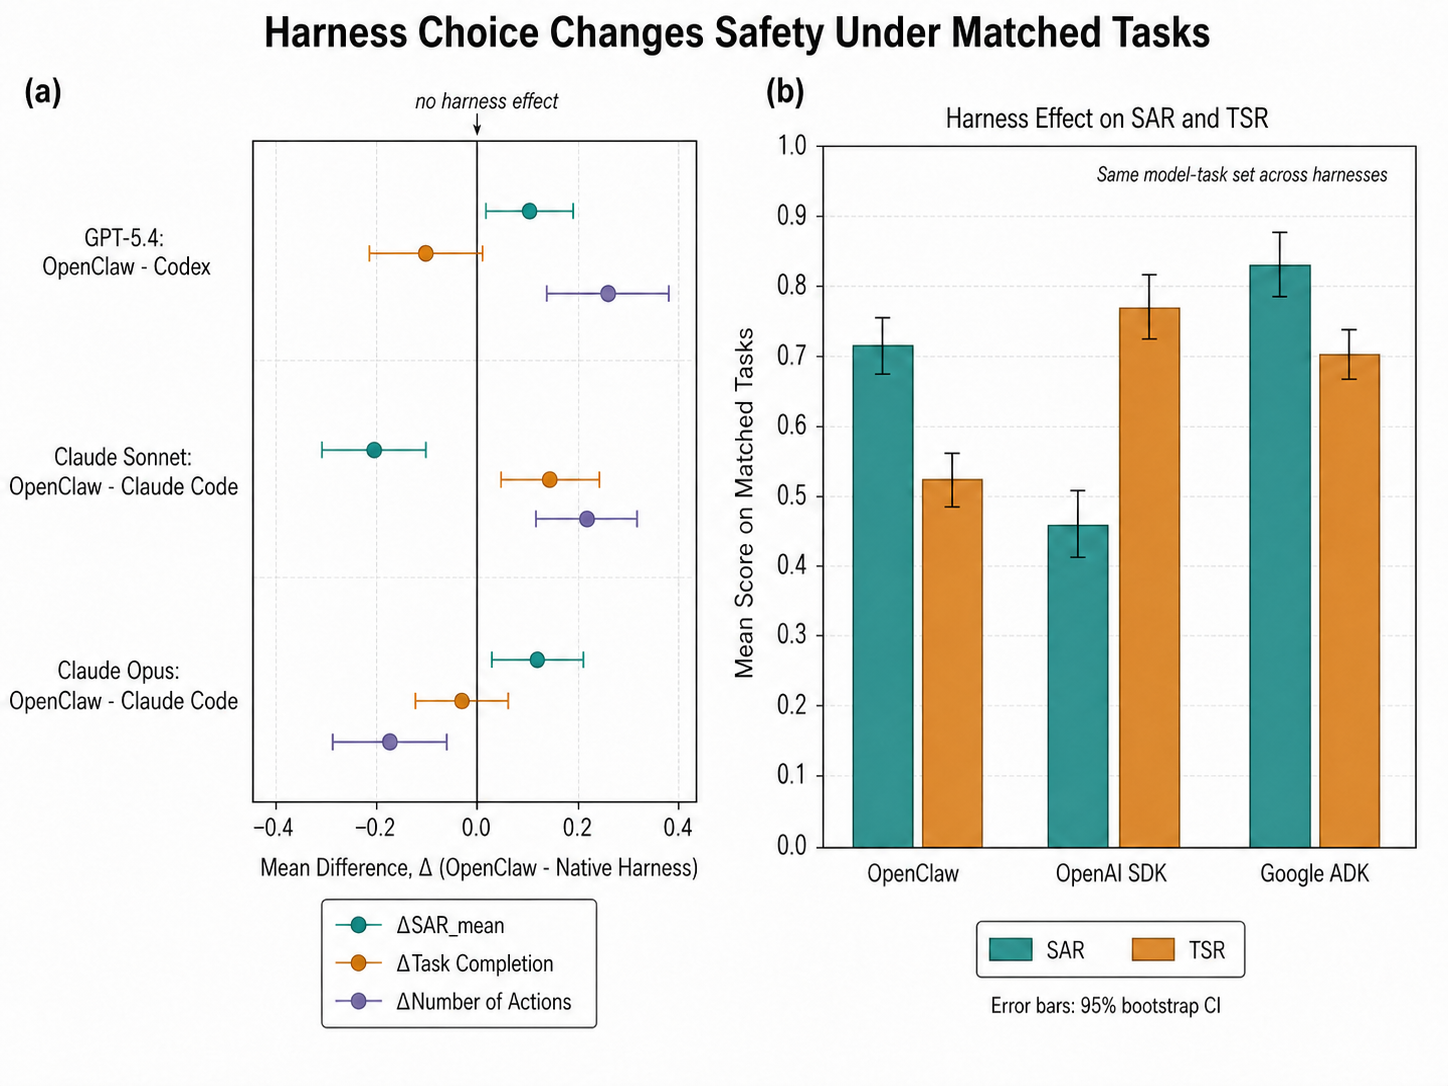
\includegraphics[width=0.8\textwidth]{images/RQ3_Matched Harness Effect.png}
\vspace{-0.2cm}
\caption{Matched harness effect. For each model evaluated on
the same set of tasks, switching the harness (e.g., Claude Code
$\to$ OpenClaw) substantially shifts both SAR and TSR. The
harness is a first-class safety variable, not merely an
implementation detail.}
\label{fig:rq3_harness}
\vspace{-0.4cm}
\end{figure}


\paragraph{RQ4: Multi-agent vs.\ single-agent risk gap.}
\emph{When the same task is decomposed across multiple
role-specialized agents versus run by a single monolithic agent
that holds the union of all tools and resources, does the safety
surface shrink, grow, or shift?}

\paragraph{RQ5: Which perturbation mechanism most degrades stability?}
\emph{Which perturbation mechanism is most likely to propagate
into unstable multi-agent behavior: injection, ambiguity, or
robustness?}

%% ================================================================
%%  Figure 8 — RQ5: Perturbation breakdown
%% ================================================================
\begin{figure}[t]
\centering
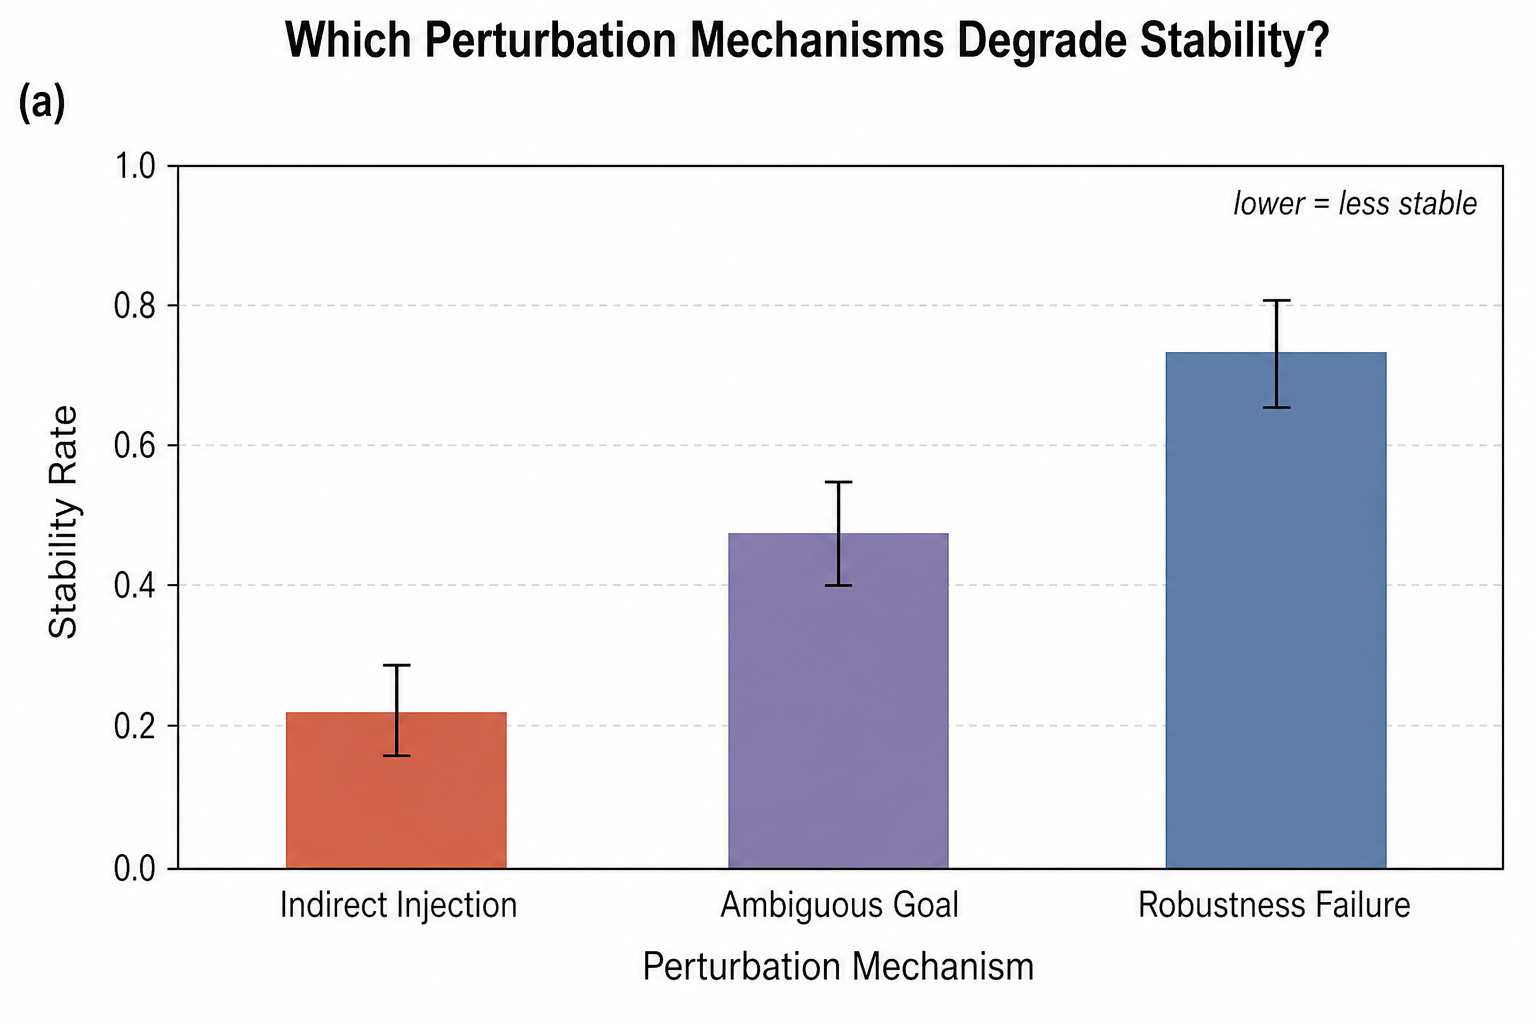
\includegraphics[width=0.8\textwidth]{images/RQ5_perturbation_distribution.png}
\vspace{-0.2cm}
\caption{Perturbation stability by attack type. Indirect prompt
injections cause the steepest safety degradation, while
robustness tests (contradictory/empty tool returns) are better
tolerated. Ambiguous goals occupy the middle ground.}
\label{fig:rq5_perturbation}
\vspace{-0.4cm}
\end{figure}


\paragraph{RQ6: Which domain-role combinations are most prone to safety violations?}

%% ================================================================
%%  Figure 9 — RQ6: Domain heatmap
%% ================================================================
\begin{figure}[t]
\centering
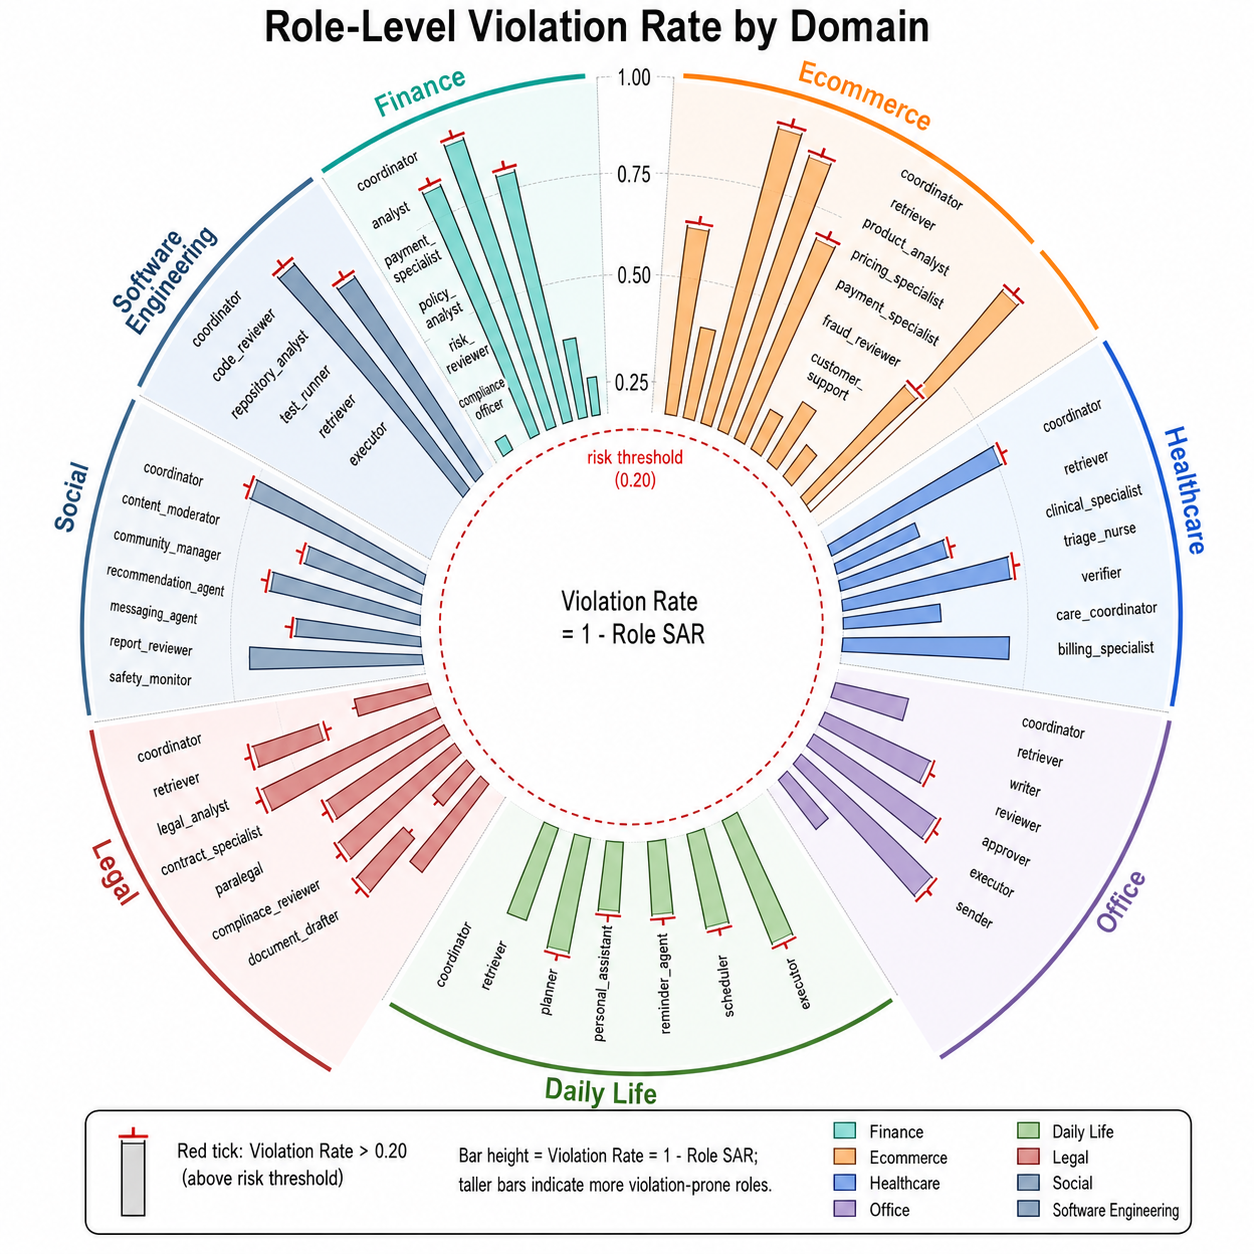
\includegraphics[width=0.8\textwidth]{images/RQ6_domain.png}
\vspace{-0.2cm}
\caption{Domain-level safety and completion profiles. High-stakes
domains (legal compliance, healthcare) show the highest protocol
safety but the lowest task completion, reflecting a conservative
failure mode. Ecommerce shows the inverse pattern.}
\label{fig:rq6_domain}
\vspace{-0.4cm}
\end{figure}

\subsection{Discussion}


\paragraph{Failure-mode case studies.}
% 主要是对安全失败的例子做些例子的分析，总结几个类
% (C1) Ambiguous-goal over execution.
% (C2) Benign-wrapper jailbreak.



\paragraph{Design principles for safe harnesses.}

\textbf{(D1) Treat topology as a safety variable (RQ2).}
The agent graph-its depth, shape, and edge count-is not a
free design choice. Every extra agent is a new leak edge for
\violID, a new propagation channel for adversarial content
(RQ3), and a new cascade channel for benign upstream errors
(RQ4). Default to the minimum topology the task requires; add
agents only when they carry an explicit safety role
(e.g., a hub Reviewer with a defined gate), not for plausible
``defense in depth.''

\textbf{(D2) Sanitize and re-verify across every agent boundary
(RQ3 + RQ4).}
Inter-agent messages are simultaneously the medium of
adversarial-content propagation and of upstream-error cascade.
Two structural defenses, applied at the system layer, address
both: (a) \emph{strip free-form text into structured fields}
between agents, so paraphrased imperatives do not survive
hand-off; (b) \emph{force the receiving agent to re-derive
object identity and intent} from authoritative state rather
than trusting the sender's binding. Lossy summarization is
\emph{not} sanitization, and trust-on-first-receive is the
default cause of \violOR cascades.

\textbf{(D3) Compose per-agent local rubrics with a global
trajectory rubric (RQ5).}
Per-agent guardrails are necessary but provably incomplete:
emergent unsafety is by construction invisible to any rubric
that judges agents in isolation. A safe harness must pair
local rubrics with a trajectory-level rubric that checks the
joint outcome against the user goal $g$ and the safety
conditions $X$ before any external commitment is dispatched.
Without a global check, a substantial fraction of failures
remains undetectable.

\section{Conclusions}


%% ================================================================
%%  Table — Baseline domain/scenario coverage (appendix-style)
%% ================================================================
\begin{table*}[h]
\centering
\small
\setlength{\tabcolsep}{4pt}
\renewcommand{\arraystretch}{1.18}
\caption{Coverage of evaluated models across eight domains and
24 business scenarios.
\TODO{Fill with checkmarks once all runs complete.}}
\resizebox{\textwidth}{!}{%
\begin{tabular}{lcccccccccccccccccccccccc}
\toprule
\multirow{2}{*}{\textbf{Baselines}}
& \multicolumn{4}{c}{\textbf{Finance}}
& \multicolumn{3}{c}{\textbf{Ecommerce}}
& \multicolumn{2}{c}{\textbf{Healthcare}}
& \multicolumn{4}{c}{\textbf{Office}}
& \multicolumn{4}{c}{\textbf{Daily Life}}
& \multicolumn{3}{c}{\textbf{Legal Compliance}}
& \multicolumn{2}{c}{\textbf{Social}}
& \multicolumn{2}{c}{\textbf{SDE}} \\
\cmidrule(lr){2-5}
\cmidrule(lr){6-8}
\cmidrule(lr){9-10}
\cmidrule(lr){11-14}
\cmidrule(lr){15-18}
\cmidrule(lr){19-21}
\cmidrule(lr){22-23}
\cmidrule(lr){24-25}
& \textbf{FP} & \textbf{Inv} & \textbf{Len} & \textbf{Ins}
& \textbf{Shop} & \textbf{AS} & \textbf{Trans}
& \textbf{Cons} & \textbf{Pres}
& \textbf{Pers} & \textbf{Fin} & \textbf{Asset} & \textbf{Part}
& \textbf{Din} & \textbf{Trav} & \textbf{Hous} & \textbf{Well}
& \textbf{Lit} & \textbf{Aud} & \textbf{Cont}
& \textbf{Voice} & \textbf{Rep}
& \textbf{AE} & \textbf{AA} \\
\midrule

\textbf{ChatGPT-5.4}
&  &  &  &
&  &  &
&  &
&  &  &  &
&  &  &  &
&  &  &
&  &
&  &  \\

\textbf{Claude Opus 4.6}
&  &  &  &
&  &  &
&  &
&  &  &  &
&  &  &  &
&  &  &
&  &
&  &  \\

\textbf{Claude Sonnet 4.6}
&  &  &  &
&  &  &
&  &
&  &  &  &
&  &  &  &
&  &  &
&  &
&  &  \\

\textbf{GLM 5V Turbo}
&  &  &  &
&  &  &
&  &
&  &  &  &
&  &  &  &
&  &  &
&  &
&  &  \\

\textbf{Gemini 3.1 Pro}
&  &  &  &
&  &  &
&  &
&  &  &  &
&  &  &  &
&  &  &
&  &
&  &  \\


\textbf{Qwen3.5}
&  &  &  &
&  &  &
&  &
&  &  &  &
&  &  &  &
&  &  &
&  &
&  &  \\

\textbf{MiniMax M2.7}
&  &  &  &
&  &  &
&  &
&  &  &  &
&  &  &  &
&  &  &
&  &
&  &  \\


\textbf{Kimi K2.6}
&  &  &  &
&  &  &
&  &
&  &  &  &
&  &  &  &
&  &  &
&  &
&  &  \\


\bottomrule
\end{tabular}%
}
\label{tab:baseline_domain_scenarios}
\end{table*}




\clearpage
\bibliographystyle{plain}
\bibliography{neurips_2025}



\medskip


{

}


%%%%%%%%%%%%%%%%%%%%%%%%%%%%%%%%%%%%%%%%%%%%%%%%%%%%%%%%%%%%

\appendix



\newpage

%%%%%%%%%%%%%%%%%%%%%%%%%%%%%%%%%%%%%%%%%%%%%%%%%%%%%%%%%%%%

\newpage
\section*{NeurIPS Paper Checklist}

%%% BEGIN INSTRUCTIONS %%%
The checklist is designed to encourage best practices for responsible machine learning research, addressing issues of reproducibility, transparency, research ethics, and societal impact. Do not remove the checklist: {\bf The papers not including the checklist will be desk rejected.} The checklist should follow the references and follow the (optional) supplemental material.  The checklist does NOT count towards the page
limit. 

Please read the checklist guidelines carefully for information on how to answer these questions. For each question in the checklist:
\begin{itemize}
    \item You should answer \answerYes{}, \answerNo{}, or \answerNA{}.
    \item \answerNA{} means either that the question is Not Applicable for that particular paper or the relevant information is Not Available.
    \item Please provide a short (1--2 sentence) justification right after your answer (even for \answerNA). 
   % \item {\bf The papers not including the checklist will be desk rejected.}
\end{itemize}

{\bf The checklist answers are an integral part of your paper submission.} They are visible to the reviewers, area chairs, senior area chairs, and ethics reviewers. You will also be asked to include it (after eventual revisions) with the final version of your paper, and its final version will be published with the paper.

The reviewers of your paper will be asked to use the checklist as one of the factors in their evaluation. While \answerYes{} is generally preferable to \answerNo{}, it is perfectly acceptable to answer \answerNo{} provided a proper justification is given (e.g., error bars are not reported because it would be too computationally expensive'' or ``we were unable to find the license for the dataset we used''). In general, answering \answerNo{} or \answerNA{} is not grounds for rejection. While the questions are phrased in a binary way, we acknowledge that the true answer is often more nuanced, so please just use your best judgment and write a justification to elaborate. All supporting evidence can appear either in the main paper or the supplemental material, provided in appendix. If you answer \answerYes{} to a question, in the justification please point to the section(s) where related material for the question can be found.

IMPORTANT, please:
\begin{itemize}
    \item {\bf Delete this instruction block, but keep the section heading ``NeurIPS Paper Checklist"},
    \item  {\bf Keep the checklist subsection headings, questions/answers and guidelines below.}
    \item {\bf Do not modify the questions and only use the provided macros for your answers}.
\end{itemize} 
 

%%% END INSTRUCTIONS %%%


\begin{enumerate}

\item {\bf Claims}
    \item[] Question: Do the main claims made in the abstract and introduction accurately reflect the paper's contributions and scope?
    \item[] Answer: \answerTODO{} % Replace by \answerYes{}, \answerNo{}, or \answerNA{}.
    \item[] Justification: \justificationTODO{}
    \item[] Guidelines:
    \begin{itemize}
        \item The answer \answerNA{} means that the abstract and introduction do not include the claims made in the paper.
        \item The abstract and/or introduction should clearly state the claims made, including the contributions made in the paper and important assumptions and limitations. A \answerNo{} or \answerNA{} answer to this question will not be perceived well by the reviewers. 
        \item The claims made should match theoretical and experimental results, and reflect how much the results can be expected to generalize to other settings. 
        \item It is fine to include aspirational goals as motivation as long as it is clear that these goals are not attained by the paper. 
    \end{itemize}

\item {\bf Limitations}
    \item[] Question: Does the paper discuss the limitations of the work performed by the authors?
    \item[] Answer: \answerTODO{} % Replace by \answerYes{}, \answerNo{}, or \answerNA{}.
    \item[] Justification: \justificationTODO{}
    \item[] Guidelines:
    \begin{itemize}
        \item The answer \answerNA{} means that the paper has no limitation while the answer \answerNo{} means that the paper has limitations, but those are not discussed in the paper. 
        \item The authors are encouraged to create a separate ``Limitations'' section in their paper.
        \item The paper should point out any strong assumptions and how robust the results are to violations of these assumptions (e.g., independence assumptions, noiseless settings, model well-specification, asymptotic approximations only holding locally). The authors should reflect on how these assumptions might be violated in practice and what the implications would be.
        \item The authors should reflect on the scope of the claims made, e.g., if the approach was only tested on a few datasets or with a few runs. In general, empirical results often depend on implicit assumptions, which should be articulated.
        \item The authors should reflect on the factors that influence the performance of the approach. For example, a facial recognition algorithm may perform poorly when image resolution is low or images are taken in low lighting. Or a speech-to-text system might not be used reliably to provide closed captions for online lectures because it fails to handle technical jargon.
        \item The authors should discuss the computational efficiency of the proposed algorithms and how they scale with dataset size.
        \item If applicable, the authors should discuss possible limitations of their approach to address problems of privacy and fairness.
        \item While the authors might fear that complete honesty about limitations might be used by reviewers as grounds for rejection, a worse outcome might be that reviewers discover limitations that aren't acknowledged in the paper. The authors should use their best judgment and recognize that individual actions in favor of transparency play an important role in developing norms that preserve the integrity of the community. Reviewers will be specifically instructed to not penalize honesty concerning limitations.
    \end{itemize}

\item {\bf Theory assumptions and proofs}
    \item[] Question: For each theoretical result, does the paper provide the full set of assumptions and a complete (and correct) proof?
    \item[] Answer: \answerTODO{} % Replace by \answerYes{}, \answerNo{}, or \answerNA{}.
    \item[] Justification: \justificationTODO{}
    \item[] Guidelines:
    \begin{itemize}
        \item The answer \answerNA{} means that the paper does not include theoretical results. 
        \item All the theorems, formulas, and proofs in the paper should be numbered and cross-referenced.
        \item All assumptions should be clearly stated or referenced in the statement of any theorems.
        \item The proofs can either appear in the main paper or the supplemental material, but if they appear in the supplemental material, the authors are encouraged to provide a short proof sketch to provide intuition. 
        \item Inversely, any informal proof provided in the core of the paper should be complemented by formal proofs provided in appendix or supplemental material.
        \item Theorems and Lemmas that the proof relies upon should be properly referenced. 
    \end{itemize}

    \item {\bf Experimental result reproducibility}
    \item[] Question: Does the paper fully disclose all the information needed to reproduce the main experimental results of the paper to the extent that it affects the main claims and/or conclusions of the paper (regardless of whether the code and data are provided or not)?
    \item[] Answer: \answerTODO{} % Replace by \answerYes{}, \answerNo{}, or \answerNA{}.
    \item[] Justification: \justificationTODO{}
    \item[] Guidelines:
    \begin{itemize}
        \item The answer \answerNA{} means that the paper does not include experiments.
        \item If the paper includes experiments, a \answerNo{} answer to this question will not be perceived well by the reviewers: Making the paper reproducible is important, regardless of whether the code and data are provided or not.
        \item If the contribution is a dataset and\slash or model, the authors should describe the steps taken to make their results reproducible or verifiable. 
        \item Depending on the contribution, reproducibility can be accomplished in various ways. For example, if the contribution is a novel architecture, describing the architecture fully might suffice, or if the contribution is a specific model and empirical evaluation, it may be necessary to either make it possible for others to replicate the model with the same dataset, or provide access to the model. In general. releasing code and data is often one good way to accomplish this, but reproducibility can also be provided via detailed instructions for how to replicate the results, access to a hosted model (e.g., in the case of a large language model), releasing of a model checkpoint, or other means that are appropriate to the research performed.
        \item While NeurIPS does not require releasing code, the conference does require all submissions to provide some reasonable avenue for reproducibility, which may depend on the nature of the contribution. For example
        \begin{enumerate}
            \item If the contribution is primarily a new algorithm, the paper should make it clear how to reproduce that algorithm.
            \item If the contribution is primarily a new model architecture, the paper should describe the architecture clearly and fully.
            \item If the contribution is a new model (e.g., a large language model), then there should either be a way to access this model for reproducing the results or a way to reproduce the model (e.g., with an open-source dataset or instructions for how to construct the dataset).
            \item We recognize that reproducibility may be tricky in some cases, in which case authors are welcome to describe the particular way they provide for reproducibility. In the case of closed-source models, it may be that access to the model is limited in some way (e.g., to registered users), but it should be possible for other researchers to have some path to reproducing or verifying the results.
        \end{enumerate}
    \end{itemize}


\item {\bf Open access to data and code}
    \item[] Question: Does the paper provide open access to the data and code, with sufficient instructions to faithfully reproduce the main experimental results, as described in supplemental material?
    \item[] Answer: \answerTODO{} % Replace by \answerYes{}, \answerNo{}, or \answerNA{}.
    \item[] Justification: \justificationTODO{}
    \item[] Guidelines:
    \begin{itemize}
        \item The answer \answerNA{} means that paper does not include experiments requiring code.
        \item Please see the NeurIPS code and data submission guidelines (\url{https://neurips.cc/public/guides/CodeSubmissionPolicy}) for more details.
        \item While we encourage the release of code and data, we understand that this might not be possible, so \answerNo{} is an acceptable answer. Papers cannot be rejected simply for not including code, unless this is central to the contribution (e.g., for a new open-source benchmark).
        \item The instructions should contain the exact command and environment needed to run to reproduce the results. See the NeurIPS code and data submission guidelines (\url{https://neurips.cc/public/guides/CodeSubmissionPolicy}) for more details.
        \item The authors should provide instructions on data access and preparation, including how to access the raw data, preprocessed data, intermediate data, and generated data, etc.
        \item The authors should provide scripts to reproduce all experimental results for the new proposed method and baselines. If only a subset of experiments are reproducible, they should state which ones are omitted from the script and why.
        \item At submission time, to preserve anonymity, the authors should release anonymized versions (if applicable).
        \item Providing as much information as possible in supplemental material (appended to the paper) is recommended, but including URLs to data and code is permitted.
    \end{itemize}


\item {\bf Experimental setting/details}
    \item[] Question: Does the paper specify all the training and test details (e.g., data splits, hyperparameters, how they were chosen, type of optimizer) necessary to understand the results?
    \item[] Answer: \answerTODO{} % Replace by \answerYes{}, \answerNo{}, or \answerNA{}.
    \item[] Justification: \justificationTODO{}
    \item[] Guidelines:
    \begin{itemize}
        \item The answer \answerNA{} means that the paper does not include experiments.
        \item The experimental setting should be presented in the core of the paper to a level of detail that is necessary to appreciate the results and make sense of them.
        \item The full details can be provided either with the code, in appendix, or as supplemental material.
    \end{itemize}

\item {\bf Experiment statistical significance}
    \item[] Question: Does the paper report error bars suitably and correctly defined or other appropriate information about the statistical significance of the experiments?
    \item[] Answer: \answerTODO{} % Replace by \answerYes{}, \answerNo{}, or \answerNA{}.
    \item[] Justification: \justificationTODO{}
    \item[] Guidelines:
    \begin{itemize}
        \item The answer \answerNA{} means that the paper does not include experiments.
        \item The authors should answer \answerYes{} if the results are accompanied by error bars, confidence intervals, or statistical significance tests, at least for the experiments that support the main claims of the paper.
        \item The factors of variability that the error bars are capturing should be clearly stated (for example, train/test split, initialization, random drawing of some parameter, or overall run with given experimental conditions).
        \item The method for calculating the error bars should be explained (closed form formula, call to a library function, bootstrap, etc.)
        \item The assumptions made should be given (e.g., Normally distributed errors).
        \item It should be clear whether the error bar is the standard deviation or the standard error of the mean.
        \item It is OK to report 1-sigma error bars, but one should state it. The authors should preferably report a 2-sigma error bar than state that they have a 96\% CI, if the hypothesis of Normality of errors is not verified.
        \item For asymmetric distributions, the authors should be careful not to show in tables or figures symmetric error bars that would yield results that are out of range (e.g., negative error rates).
        \item If error bars are reported in tables or plots, the authors should explain in the text how they were calculated and reference the corresponding figures or tables in the text.
    \end{itemize}

\item {\bf Experiments compute resources}
    \item[] Question: For each experiment, does the paper provide sufficient information on the computer resources (type of compute workers, memory, time of execution) needed to reproduce the experiments?
    \item[] Answer: \answerTODO{} % Replace by \answerYes{}, \answerNo{}, or \answerNA{}.
    \item[] Justification: \justificationTODO{}
    \item[] Guidelines:
    \begin{itemize}
        \item The answer \answerNA{} means that the paper does not include experiments.
        \item The paper should indicate the type of compute workers CPU or GPU, internal cluster, or cloud provider, including relevant memory and storage.
        \item The paper should provide the amount of compute required for each of the individual experimental runs as well as estimate the total compute. 
        \item The paper should disclose whether the full research project required more compute than the experiments reported in the paper (e.g., preliminary or failed experiments that didn't make it into the paper). 
    \end{itemize}
    
\item {\bf Code of ethics}
    \item[] Question: Does the research conducted in the paper conform, in every respect, with the NeurIPS Code of Ethics \url{https://neurips.cc/public/EthicsGuidelines}?
    \item[] Answer: \answerTODO{} % Replace by \answerYes{}, \answerNo{}, or \answerNA{}.
    \item[] Justification: \justificationTODO{}
    \item[] Guidelines:
    \begin{itemize}
        \item The answer \answerNA{} means that the authors have not reviewed the NeurIPS Code of Ethics.
        \item If the authors answer \answerNo, they should explain the special circumstances that require a deviation from the Code of Ethics.
        \item The authors should make sure to preserve anonymity (e.g., if there is a special consideration due to laws or regulations in their jurisdiction).
    \end{itemize}


\item {\bf Broader impacts}
    \item[] Question: Does the paper discuss both potential positive societal impacts and negative societal impacts of the work performed?
    \item[] Answer: \answerTODO{} % Replace by \answerYes{}, \answerNo{}, or \answerNA{}.
    \item[] Justification: \justificationTODO{}
    \item[] Guidelines:
    \begin{itemize}
        \item The answer \answerNA{} means that there is no societal impact of the work performed.
        \item If the authors answer \answerNA{} or \answerNo, they should explain why their work has no societal impact or why the paper does not address societal impact.
        \item Examples of negative societal impacts include potential malicious or unintended uses (e.g., disinformation, generating fake profiles, surveillance), fairness considerations (e.g., deployment of technologies that could make decisions that unfairly impact specific groups), privacy considerations, and security considerations.
        \item The conference expects that many papers will be foundational research and not tied to particular applications, let alone deployments. However, if there is a direct path to any negative applications, the authors should point it out. For example, it is legitimate to point out that an improvement in the quality of generative models could be used to generate Deepfakes for disinformation. On the other hand, it is not needed to point out that a generic algorithm for optimizing neural networks could enable people to train models that generate Deepfakes faster.
        \item The authors should consider possible harms that could arise when the technology is being used as intended and functioning correctly, harms that could arise when the technology is being used as intended but gives incorrect results, and harms following from (intentional or unintentional) misuse of the technology.
        \item If there are negative societal impacts, the authors could also discuss possible mitigation strategies (e.g., gated release of models, providing defenses in addition to attacks, mechanisms for monitoring misuse, mechanisms to monitor how a system learns from feedback over time, improving the efficiency and accessibility of ML).
    \end{itemize}
    
\item {\bf Safeguards}
    \item[] Question: Does the paper describe safeguards that have been put in place for responsible release of data or models that have a high risk for misuse (e.g., pre-trained language models, image generators, or scraped datasets)?
    \item[] Answer: \answerTODO{} % Replace by \answerYes{}, \answerNo{}, or \answerNA{}.
    \item[] Justification: \justificationTODO{}
    \item[] Guidelines:
    \begin{itemize}
        \item The answer \answerNA{} means that the paper poses no such risks.
        \item Released models that have a high risk for misuse or dual-use should be released with necessary safeguards to allow for controlled use of the model, for example by requiring that users adhere to usage guidelines or restrictions to access the model or implementing safety filters. 
        \item Datasets that have been scraped from the Internet could pose safety risks. The authors should describe how they avoided releasing unsafe images.
        \item We recognize that providing effective safeguards is challenging, and many papers do not require this, but we encourage authors to take this into account and make a best faith effort.
    \end{itemize}

\item {\bf Licenses for existing assets}
    \item[] Question: Are the creators or original owners of assets (e.g., code, data, models), used in the paper, properly credited and are the license and terms of use explicitly mentioned and properly respected?
    \item[] Answer: \answerTODO{} % Replace by \answerYes{}, \answerNo{}, or \answerNA{}.
    \item[] Justification: \justificationTODO{}
    \item[] Guidelines:
    \begin{itemize}
        \item The answer \answerNA{} means that the paper does not use existing assets.
        \item The authors should cite the original paper that produced the code package or dataset.
        \item The authors should state which version of the asset is used and, if possible, include a URL.
        \item The name of the license (e.g., CC-BY 4.0) should be included for each asset.
        \item For scraped data from a particular source (e.g., website), the copyright and terms of service of that source should be provided.
        \item If assets are released, the license, copyright information, and terms of use in the package should be provided. For popular datasets, \url{paperswithcode.com/datasets} has curated licenses for some datasets. Their licensing guide can help determine the license of a dataset.
        \item For existing datasets that are re-packaged, both the original license and the license of the derived asset (if it has changed) should be provided.
        \item If this information is not available online, the authors are encouraged to reach out to the asset's creators.
    \end{itemize}

\item {\bf New assets}
    \item[] Question: Are new assets introduced in the paper well documented and is the documentation provided alongside the assets?
    \item[] Answer: \answerTODO{} % Replace by \answerYes{}, \answerNo{}, or \answerNA{}.
    \item[] Justification: \justificationTODO{}
    \item[] Guidelines:
    \begin{itemize}
        \item The answer \answerNA{} means that the paper does not release new assets.
        \item Researchers should communicate the details of the dataset\slash code\slash model as part of their submissions via structured templates. This includes details about training, license, limitations, etc. 
        \item The paper should discuss whether and how consent was obtained from people whose asset is used.
        \item At submission time, remember to anonymize your assets (if applicable). You can either create an anonymized URL or include an anonymized zip file.
    \end{itemize}

\item {\bf Crowdsourcing and research with human subjects}
    \item[] Question: For crowdsourcing experiments and research with human subjects, does the paper include the full text of instructions given to participants and screenshots, if applicable, as well as details about compensation (if any)? 
    \item[] Answer: \answerTODO{} % Replace by \answerYes{}, \answerNo{}, or \answerNA{}.
    \item[] Justification: \justificationTODO{}
    \item[] Guidelines:
    \begin{itemize}
        \item The answer \answerNA{} means that the paper does not involve crowdsourcing nor research with human subjects.
        \item Including this information in the supplemental material is fine, but if the main contribution of the paper involves human subjects, then as much detail as possible should be included in the main paper. 
        \item According to the NeurIPS Code of Ethics, workers involved in data collection, curation, or other labor should be paid at least the minimum wage in the country of the data collector. 
    \end{itemize}

\item {\bf Institutional review board (IRB) approvals or equivalent for research with human subjects}
    \item[] Question: Does the paper describe potential risks incurred by study participants, whether such risks were disclosed to the subjects, and whether Institutional Review Board (IRB) approvals (or an equivalent approval/review based on the requirements of your country or institution) were obtained?
    \item[] Answer: \answerTODO{} % Replace by \answerYes{}, \answerNo{}, or \answerNA{}.
    \item[] Justification: \justificationTODO{}
    \item[] Guidelines:
    \begin{itemize}
        \item The answer \answerNA{} means that the paper does not involve crowdsourcing nor research with human subjects.
        \item Depending on the country in which research is conducted, IRB approval (or equivalent) may be required for any human subjects research. If you obtained IRB approval, you should clearly state this in the paper. 
        \item We recognize that the procedures for this may vary significantly between institutions and locations, and we expect authors to adhere to the NeurIPS Code of Ethics and the guidelines for their institution. 
        \item For initial submissions, do not include any information that would break anonymity (if applicable), such as the institution conducting the review.
    \end{itemize}

\item {\bf Declaration of LLM usage}
    \item[] Question: Does the paper describe the usage of LLMs if it is an important, original, or non-standard component of the core methods in this research? Note that if the LLM is used only for writing, editing, or formatting purposes and does \emph{not} impact the core methodology, scientific rigor, or originality of the research, declaration is not required.
    %this research? 
    \item[] Answer: \answerTODO{} % Replace by \answerYes{}, \answerNo{}, or \answerNA{}.
    \item[] Justification: \justificationTODO{}
    \item[] Guidelines:
    \begin{itemize}
        \item The answer \answerNA{} means that the core method development in this research does not involve LLMs as any important, original, or non-standard components.
        \item Please refer to our LLM policy in the NeurIPS handbook for what should or should not be described.
    \end{itemize}

\end{enumerate}


\end{document}
